\chapter{Architecture} \label{CH:architecture}

\section{Architectural Overview}\label{sec:arch:overview}
The goal of the Torchbearer system is simple: given the latitude, longitude and approach bearing of a maneuver point, render a string describing the most salient landmark at that location. The problem which Torchbearer solves the problem expressed by
\begin{equation}\label{eq:problem}
    f(lat, long, bearing) \longrightarrow description
\end{equation}
where $f$ is some method of landmark selection and description. The Torchbearer system provides multiple implementations of $f$, which we call pipelines. Each pipeline consists of an ordered set of tasks, $T$. Each task $t_i \in T$ accepts some input from the previous task $t_{i-1}$ and returns some output to be input to the next task $t_{i+1}$---the obvious exceptions being the first task, which takes a tuple $(lat, long, bearing)$ as input, and the last task, which outputs the selected landmark---the final result of the pipeline. Each task progressively solves a small part of the landmark selection problem, such that at the end of the pipeline Torchbearer has computed a lexical description of the most suitable landmark. It is natural to consider a pipeline as a composition of functions:
\begin{equation}\label{eq:pipeline}
    P=t_{n-1} \dots t_1(t_0(lat, long, bearing)) \longrightarrow description
\end{equation}
where $n = \mid T \mid$. As an implementation detail, it is important to note that tasks can be performed in parallel if they all take the same input form the previous task. Examples of such parallelization are shown in the descriptions of each specific pipeline.

\begin{figure}[htbp]
  \centering
  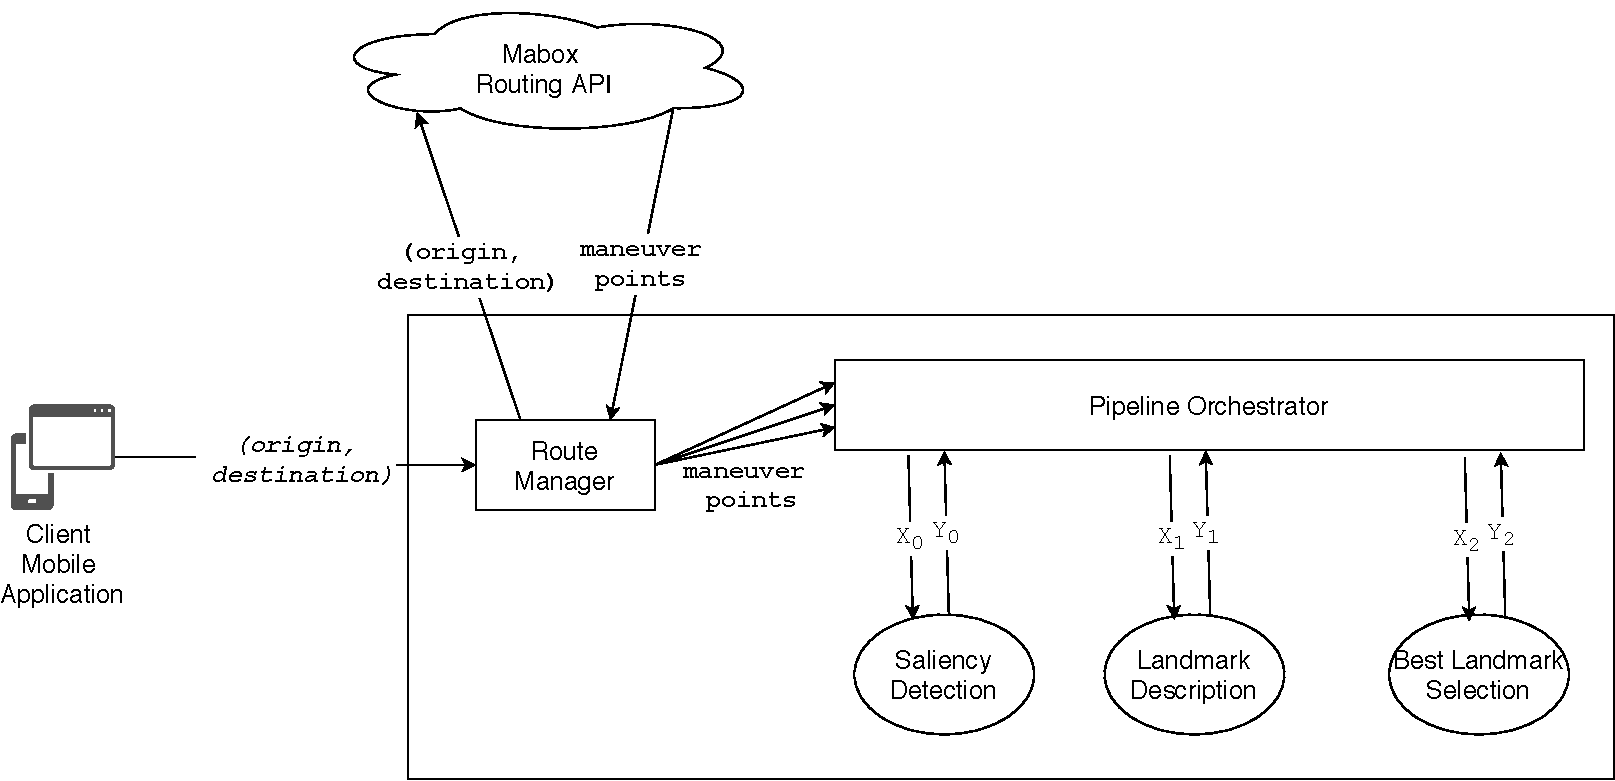
\includegraphics[width=\textwidth]{images/Arch.pdf}
  \caption{A high-level view of the Torchbearer system.}
  \label{fig:pipeline:overview}
\end{figure}

The Torchbearer system receives input from a client mobile application in the form of a $(origin, destination)$ tuple. After gathering a set of maneuver points from the Mapbox Routing API, the Orchestrator receives a list of $(latitude, longitude, bearing)$ tuples corresponding to each maneuver point for which a landmark description should be computed. The Orchestrator manages the execution of each Task in the pipeline, and returns the final selected landmark to be saved in a database, where it can be queried by the mobile client. We discuss each component of the system in further detail below.

\section{Orchestration}\label{sec:arch:orchestration}
In order to implement the function composition approach discussed above, each pipeline requires a system to progress a maneuver point through each task in the pipeline. We call such a system the pipeline’s \textit{Orchestrator}. The Orchestrator is the manifestation of the pipeline, in the sense that it is solely responsible for the intake of new maneuver points to be processed and overseeing the ordered execution of each task for that maneuver point.

The Orchestrator is centralized service which acts as a specialized message broker. For each task $t$ in the pipeline, the Orchestrator maintains a FIFO queue $q_t$ of maneuver points for processing through that task. Queue items are tulpes containing the unique identifier of the maneuver point, a token representing the specific task instance and the input to the given task, $I_t$.

A task \textit{worker}, described in the next section, polls the Orchestrator for a task in need of completion; if such a task is available the Orchestrator pops it the from queue and returned to the worker. (We discuss polling in greater detail in the following section.) When the worker has the completed the task, it sends the results back to the Orchestrator, which then adds a new item to the queue corresponding to the next task $t_+$, including the output of $t$ (which is the input to $t_+$). If the execution of the task results in an error, the worker sends the details of the error to the Orchestrator, which then halts further execution of the pipeline for that maneuver point.

The Orchestrator supports parallel execution of tasks, by placing a maneuver point into two queues simultaneously, and pausing progression of the pipeline until \textbf{both} tasks complete. The input $X$ to the next task $t+1$ is then the union of the outputs of the $n$ parallel tasks:
\begin{equation}\label{eq:paraOrch}
    X_{t+1} = Y_0 \cup Y_1 \dots \cup Y_n
\end{equation}

An Orchestrator also maintains a database of pipeline state, including, for each maneuver point, the output of each task, or error details if one occurred. The execution for a specific point can be traced or monitored throughout the pipeline by querying this database.

\section{Task Implementation}\label{sec:arch:pipeline_imp}
A task receives a tuple $X$ as its input and yields a tuple $Y$ as its output. A task’s output must be inclusive of its inputs, that is, $X \subset Y$. Let $p_+ = Y \setminus X$, then $p_+$ is the context contribution of a given task---the information which that state has added to the pipeline's overall knowledge, or state. For example, a task devoted to describing landmarks might receive a list of candidate landmarks as input, and output both that list and a list of computed descriptions for each landmark.

It is important to note that each task has a binding contract in terms of its input and output, based on where it sits in the pipeline. For example, task $t_1$ must accept input corresponding to the output of task $t_0$, and must provide output corresponding to the input to task $t_2$. This contract presents a not insignificant constraint in regards to rearranging tasks within a pipeline: even if $t_1(t_2) == t_2(t_1)$ (that is, the order in which the pair of tasks is executed is not important) the two tasks could not change positions in the ordered set of tasks for the pipeline unless their inputs and outputs were identical. 

A task is solved by a worker. A worker is an independent, isolated computational entity which is responsible for the execution of a specific task. There can be any number of (identical) workers for a task active at one time, essentially functioning as a cluster, allowing for multiple instances of the given task to be executed simultaneously. (Each instance of a task will only be run on one worker.) For example, multiple worker instances for the Landmark Description task could run at the same time, allowing for parallel execution.

Workers are stateless: in order to complete its task, a worker relies only on the input it receives from the Orchestrator, without regard to previous tasks completed by other workers. To describe a landmark, for example, the Landmark Description worker does not require any information about other landmarks within the Torchbearer system.  Workers have no awareness of the context in which they do their jobs, in the sense that workers can handle tasks from multiple pipelines and do not care about the order in which they are asked to handle tasks. 

A worker performs three essential functions: first, to find new tasks needing execution, it polls the pipeline Orchestrator. Second, it carries out the computational operations needed to complete the task, utilizing inputs from the Orchestrator. Lastly, it returns outputs to the Orchestrator upon successful completion of the task, or alerts the Orchestrator of a failure. 
 
\subsection{Polling for Tasks}
The first function of a worker is to poll pipeline Orchestrators for tasks in need of completion. A worker will ask only for the task or tasks it is capable of executing. It is important to note that the Orchestrator utilizes a pull mechanism for task assignment, as opposed to a push mechanism: rather than Orchestrators routing tasks to specific Workers, each Worker is responsible for “finding” its own work by asking Orchestrators for available jobs. While an Orchestrator serves as a manager for tasks, having state related to the precise status of all pending tasks in its pipeline, it does not serve as a manager for Workers. Indeed, no component of the Torchbearer system maintains state related to the Worker pool. Workers can be stood up or can fail without disruption.

The polling mechanism runs within its own thread and runs in a continuous loop. Each iteration of the loop consists of the following: to initiate the polling sequence, a Worker sends an HTTP GET request to the Orchestrator. If the Orchestrator has any tasks which the worker is capable of completing, it immediately responds with a payload containing a list of tuples, where each tuple contains inputs and a unique identifier corresponding to each specific task. If no such task is currently available, the Orchestrator holds the request open for up to 60 seconds, waiting for a task to become available. As soon as a task becomes available the payload is sent and the request ended. If no task becomes available during the 60 second window, the Orchestrator terminates request with an empty response.

When a worker receives a response from the polling request, it first checks to see if the response contains a payload (indicating that at least one task was received.) If the response contains a payload, it spawns a thread for each received task to process (complete) the given task, passing in the input and unique identifier received from the payload. If the response does not contain a payload, the current iteration of the loop completes, and the process repeats with a new polling request immediately being invoked.

\subsection{Task Execution}

The execution step is responsible for solving or completing the worker’s task. The majority of this step’s procedure depends on the task, and is discussed for each task in depth later on. It is important at this juncture to understand only that the execution step for a given task runs asynchronously in its own thread, spawned by the polling thread and being provided with both the inputs to the task and unique identifier of the task. The runnable routine of this thread consists of a program which will accept the task’s inputs and yield the task’s outputs--that is, it solves or completes the task. 

\subsection{Submitting Results}

If the task completes successfully, the task execution thread sends an HTTP POST request to the Orchestrator, consisting of the task token as well as the yielded output. If any error occurred during execution, the worker sends an HTTP POST request to the Orchestrator containing the task token, the error message and any additional data about the error, such as a stack trace.

\section{Worker Deployment and Operations}
Torchbearer is a microservice-based system; workers have complete flexibility in implementation. Besides conforming to the input/output contract specific for the given task, Torchbearer is entirely agnostic to how a worker completes its task and where (on what machine) it does so. This flexibility provides incredible power in terms of optimizing compute resources and designing solutions which are best-suited to a particular task. Workers can implement solutions, in any language, run on any operating system and run on hardware suited to their particular demands. For example, we implement a task for looking up a location in GIS database in Scala, and, due to its lightweight computational demands, it runs on a single-core machine with 256 MB of RAM. On the other hand, we implement a deep neural network-based computer vision task in Python, and run it on a multi-core machine with a 3072-core GPU and 16 GB of RAM.

In order to facilitate this level of microservice-based independence, Torchbearer we implement Torchbearer workers as Docker containers and run them on Amazon's Elastic Container Service (ECS). A Docker container enables a worker to define the exact specifications for a virtual machine, and ECS runs this container on an appropriate hardware node. The container is a self-contained bundle consisting of the virtual machine definition and the binary for the worker program (the code which actually handles the task.) 

By containerizing workers and running them on a container management service such as ECS we also gain the ability to horizontally and vertically scale compute resources at the task/worker level. We can run multiple instances of each container simultaneously, and we can adjust the number of instances in real time according to changing demands for a service---this provides us with horizontal scalability. For example, a task utilized by every pipeline will, in the steady-state, require more instances than one which is used by only a single pipeline. Since the demand for Torchbearer’s services is in constant flux (in general, a higher number of active users corresponds to a higher load requirement) the ability to add and remove instances of a worker as the demand for that task fluctuates is highly important to the cost-effectiveness and efficiency of the system.

\section{Route Manager}
The Route Manager (RM) service is the contact point between the Torchbearer backend and users (via the client mobile application, discussed below.) While the RM service is not directly responsible for solving the landmark description problem, RM serves as the gateway for client applications wishing to use the Torchbearer system. RM exposes a public-facing Application Programming Interface (API) consisting of the following endpoints:

\subsection{POST /route}
A client (generally an end user's mobile phone) calls this endpoint both to determine the shortest-path route to a destination as well as to initiate landmark processing in the Torchbearer system. This endpoint accepts an origin tuple consisting of $(latitude, longitude)$ (generally, the user's current location) as well as a destination tuple of the same form, and returns the shortest-path route in the form a list of maneuver points. A maneuver point is a tuple consisting of the latitude, longitude, and bearing of the maneuver, the unique ID of the maneuver point within the Torchbearer system and and an instruction to be spoken to the user as they near that maneuver point. If immediately available, the tuple also includes the landmark description computed by the specified pipeline; we discuss this in more detail shortly.

When RM receives this type of request, it must first determine the shortest-path route between the origin and destination points. We use Mapbox, a third-party service which offers a public street routing API. While there are no special requirements for the routing algorithm Torchbearer uses, Mapbox was chosen for its unique trait of including approach bearings for each maneuver point. Another routing service, or a custom solution, could be integrated into Torchbearer in place of Mapbox, so long as it accepts origin and destination coordinates as input and returns a list of maneuver points, each consisting of latitude, longitude, approach bearing and maneuver type (right turn, left turn, merge, etc.)

Once the route has been determined, RM queries the Torchbearer database for each maneuver point. If the maneuver point exists in the Torchbearer system, and has already been processed by the specified pipeline, the computed landmark description is returned in the response. If the maneuver point does not exist, RM inserts a record for it into the database, and initiates processing by sending an HTTP POST request to the Orchestrator of the desired pipeline. The list of maneuver points are then returned to the client.

It is important to note that while this endpoint will immediately return all maneuver points for a route, some maneuver points will be in a processing state (by the given pipeline). If a point is still processing, RM returns it without a landmark description, and the client will need to ask RM for an updated description at later time using the \texttt{GET /maneuverpoint/landmark} endpoint.

\subsection{GET /maneuverpoint/landmark}
This endpoint accepts a maneuver point’s unique identifier and a pipeline as input and returns a description of the landmark computed for that maneuver point using that pipeline, if one is available. This endpoint is used for checking if Torchbearer has completed processing a maneuver point after the initial route has been returned. For example, if a client navigation application did not yet know the landmark description for an upcoming maneuver point, it might query this endpoint immediately prior to speaking a navigation instruction, to see if a landmark description was now available.

\section{User Interface}\label{sec:arch:ui}
Users interact with Torchbearer via a native mobile application, developed for both iOS and Android devices. The application has two principal functionalities: first, the ability to search for a destination and submit the route to the Torchbearer system, second, the delivery of spoken turn-by-turn navigation instructions containing the landmark description-based instructions created by one of Torchbearer’s pipelines.

Usage of the application during a typical navigation consists of the following flow: first, the user selects the pipeline they wish to use for computing instructions. By default, the application selects the machine-machine pipeline, which we discuss in a subsequent section. Second, the user enters a desired destination using the keyboard or text-to-speech capability of her device. The destination can be an address, business, point-of-interest, or general area, such as a city. Using geocoding services provided by Google, the application determines the most relevant geographical coordinates for the destination description entered by the user. The geocoding service takes into account the provided description and the user's current location in determining the most likely destination. The app displays the address derived by the geocoding service to the user, and asks her to confirm its correctness.

After confirmation from the user, the application submits an HTTP POST request to Torchbearer's Route Manager service, which returns a list of instruction tuples for the route. Each tuple consists of the coordinates of the maneuver point as well as the instruction string for the app to "speak" upon approaching the turn. While this response is returned immediately, the processing of the route (to determine landmark descriptions) is asynchronous. If a maneuver point has already been processed by the specified pipeline, its full instruction can be immediately returned in the response, but for points not yet analyzed by the pipeline, only the street name can be returned. As such, the initial route received by the application may not contain complete instructions, that is, instructions inclusive of landmark descriptions, for all maneuver points. 

At this point, the application delivers a spoken instruction to the user for the first maneuver point in the route, and the user begins driving. This begins the \textit{check-speak-repeat} loop: at a distance of one-half mile from the proximate maneuver point, the application checks whether it received a landmark description for the maneuver point from Route Manager, as part of the initial route request. If not, it sends an HTTP GET request to Route Manager seeking an updated instruction. If the processing for the maneuver point is now complete, Route Manager responds with the updated instruction. 

At a distance of one-quarter mile from the maneuver point, the application alerts the user to the upcoming maneuver via a spoken direction of the form \textit{``in one-quarter mile, [action] at the [landmark] onto [street]"} where \textt{action} is a predefined description of the maneuver to be performed, such as “turn right” or “merge”, \texttt{landmark} is the landmark description computed by Torchbearer, and \texttt{street} is the name of the street onto which the maneuver will take the user. In the case where no landmark description is available, either because the pipeline did not finish processing the maneuver point in time or was unable to compute a description, the ``at the [landmark]" portion of the instruction is omitted. At a distance of 25-feet the application will speak an instruction of the form ``[action] at the [landmark] onto [street]". When the user passes through the maneuver point, executing the maneuver, the \textit{check-speak-repeat} iteration for the current maneuver is complete.

While the \textit{check-speak-repeat} routine is the same for alerting the user of arrival at their final destination as for intermediate maneuver points, the delivery varies slightly: immediately after completing the second-to-last maneuver (the last maneuver being arrival at the destination) the application speaks an instruction of the form \textit{``In [distance] your destination is the [landmark] on the [side] of the street"} where \texttt{side} is either ``left" or ``right".

Upon arrival at the destination, the application speaks one last instruction of the form ``you have arrived at your destination. It's the [landmark] on the [side]." The arrival event completes the navigation session, and the application returns to a point from which the user can enter a new destination and begin a new session.

The mobile application is implemented using the React Native framework \cite{reactNative}, a cross-platform, JavaScript-based library. This framework allows for a single codebase across both iOS and  Android, and while it is written in JavaScript as opposed to the native Swift or Java, all visual components are rendered natively on the device. This creates a highly-responsive interface that feels like a native application as opposed to a mobile website. 

\section{Street-level Imagery}
Much of Torchbearer's work, whether human-based or machine-based, relies on visual computations based on the visual scene a driver would be seeing as he approaches a maneuver point. This computation requires a source of street-level imagery, photographs, taken from a vehicle on the road. These images must be of a relatively high definition (at least 640 pixels by 640 pixels), be in color and be available at all maneuver points through which Torchbearer provides navigation services (ideally, most roadways in the United States). Additionally, images must have no distortion, either by attribute of camera setup or post-production correction. That is, each image much be rectilinear.

We use Google Street View due its high coverage of U.S. roads, high definition images, and public availability. The service can return an image for a particular latitude, longitude and compass bearing. The service returns rectilinear-projected \cite{agarwal2015metric}, distortion free images for a given latitude, longitude, field of view and bearing. Field of view is limited to 120 degrees, as any larger can lead to incorrect perspective near the vertical edges of the image---a side effect of rectilinear projection.
 
\section{Human Input}
Torchbearer makes decisions via two means---algorithms and humans. Leveraging human opinion and decision-making in a computational system presents unique challenges, which are not considerations in most computer systems. Human input provides Torchbearer with insight into the landmark description problem that may be difficult to express algorithmically: while our machine-based pipelines include well-founded heuristics for finding and describing the best landmark to use for describing a maneuver point, we hypothesize that humans may offer some unique insight into solving this problem that our heuristics do not. The subjective nature of determining the “best” landmark, as well as a description of what that landmark is, make human insight and opinion especially valuable. 

In order to gather human input at a large scale, in real time, we require a large source of human workers. For this Torchbearer leverages Mechanical Turk (MTurk), a large-scale crowdsourcing platform. Mechanical Turk manages a pool of workers, and allows requesters (such as Torchbearer) to submit Human Intelligence Tasks (HITs) to this pool. At a high level, a HIT is simply a question to be asked of a human worker, with some form of answer specification. Torchbearer presents HITs to workers via a web page hosted on its servers, allowing for rich content to be displayed to the worker.

Each HIT specifies a monetary reward, which Torchbearer pays to the worker upon successful completion of the HIT, as well as a maximum duration the worker is allowed to work on the HIT. Additionally, the HIT can demand that the worker has a certain qualification---a test created by Torchbearer, which the worker must pass---in order to be allowed to work on the HIT.  Lastly, the HIT specifies how many workers it should be completed by, allowing for the collection of multiple answers to the same question. When a HIT is submitted to MTurk, it becomes available for workers to complete. Workers choose the HITs they work on; they are not automatically assigned. Once a HIT has been completed by the specified number of workers, the answers are sent back to the requester by adding them to a distributed queue.

While each human-based pipeline task specifies its own format for questions and answers, the general system Torchbearer uses for gathering data via MTurk is constant. When a pipeline task requests human input, Torchbearer's MTurk management service (Turk Service) submits a HIT to MTurk with the parameters specified by the pipeline task. Some questions are simple in terms of how they can be displayed to the worker. They may consist of a text-based question with text-based answers, for example. Such questions are submitted to MTurk as part of the HIT specification, and are hosted entirely by MTurk. (The Description Verification task, which we discuss in detail later on, is an example of this type of HIT.) Other questions may require displaying rich content to the worker and accepting interactive answers, such as the drawing of boxes around landmarks in an image. These questions must be served to workers as HTML pages by Turk Service, and the HIT only specifies the URL of the given page. When a worker is ready to complete the task, MTurk requests the page from Turk Service, and displays it to the worker.

MTurk collects answers from workers as they complete each HIT. Once a HIT has been completed by the number of workers required, MTurk sends the list of answers back to Torchbearer by adding a message to a distributed queue shared between Torchbearer and MTurk. Turk Service continuously polls this queue for new lists of answers. When one arrives, Turk Service first determines the aggregated answer---the final answer based on a combination of the individual answers of each worker---by applying an aggregation function. (The aggregation function varies by HIT; we discuss the specific function for each human-based task in the Pipelines section.) Turk Service sends this aggregated answer to the Orchestrator of the pipeline, and pipeline execution continues.

\subsection{Getting Meaningful Answers}

The primary challenge associated with asking a question of a worker is that of trust: do we trust that the worker gave us a meaningful answer, that she took the time to give the best response, as opposed to the easiest? Additionally, do we trust that she actually understood the task? 

In the simplest scenario, for a specific human input question, Torchbearer submits a single HIT to MTurk, and accepts the response from the worker who completed it as the final answer. While straightforward, this approach does not offer confidence in how meaningful the response is---it is possible the worker put minimum effort into the HIT in the name of speedy completion. To counteract this, Torchbearer makes use of two separate methods for filtering out nonsensical human answers: sampling and majority verification. Additionally, we require that all MTurk workers complete a training exercise and pass a qualification test specific to the task they are working on prior to submitting any results. The training materials and examination are hosted by MTurk.

\subsubsection{Worker Qualification}

Leveraging MTurk's Qualification system allows us to filter out workers who do not understand the goal of Torchbearer's HITs. This screening allows us to both train the worker in how to complete a task as well as ensure they have the understanding and insight needed to complete the task successfully. While qualification does not prevent a worker from providing (either intentionally or unintentionally) a bad answer, it does ensure that they are capable of providing an answer of acceptable quality.

The qualification system consists of two components, training and enforcement. The training component consists of a web-based guide to completing the given task, complete with good and bad examples, descriptions of the goal of the task and step-by-step instructions. When a worker first desires to work on a Torchbearer HIT, she is presented with this guide. After viewing it, she may take the qualification test, a short multiple-choice exam which asks the worker to pick the best answer to an example HIT. Even though some questions may be largely opinion-based, the answer set is clear as to which choice would be an acceptable answer. Other answers have a glaring inconsistency which the guide would have specifically pointed out as being undesirable--such as selecting a non-permanent object as the best landmark. An example test can be seen in Appendix \ref{appendix:qual}.

In order to be allowed to work on Torchbearer HITs, a worker must score at least 80\% on the qualification test and have viewed all parts of the training guide. Until these requirements have been met for a given type of HIT, MTurk will not allow the worker to submit answers. 

\subsubsection{Sampling}

In the sampling approach, we require that multiple workers complete each HIT, providing us with multiple responses. We can then determine the final answer by applying an aggregation function to the individual responses, such as taking the mean or median or mode. 

We benefit in two ways from this approach: first, having a majority of meaningful responses dampens the response of a negligent worker. Consider the trivial example of a HIT asking workers to count the number of cars appearing in an image. If we asked only a single worker, we would have to take her at her word, with no means of knowing how correct or incorrect her response was. However, if we ask five workers, and three provide the correct count while two provide the incorrect count (whether by intentional neglect or honest mistake) we could still arrive at the correct answer by either taking the median or the mode. Of course, the increased cost of this approach is directly proportional to the number of workers we ask to complete our HIT.

The second benefit comes into play if there is more than one answer to the question being asked, or if the question is largely opinion-based. Consider an example where we want to know which car in an image is the nicest, or most luxurious. Obviously, this is not an objective question--but we may still be able to gain insight by looking at the most frequent answers given by our sample of workers. If four workers suggest that car A is the nicest, one suggests that car B is the nicest, and one suggest that it is in fact car C, then we have reasonable evidence that car A is considered to be the most luxurious.

The sampling approach is powerful, but works best when the answers are quantitative and can be easily aggregated. For HITs which require answers that are difficult to aggregate and compare the majority verification approach is best.

\subsubsection{Majority Verification}

Instead of requiring multiple workers to answer each HIT, the majority verification approach, inspired by Kulkarni et al. \cite{kulkarni2011turkomatic}, requires only one answer. However, to ensure that the given answer is correct, a sample of workers (generally three) is asked to confirm that the answer is correct. This verification is treated as a majority vote: if at least two out of three workers assert that the given answer is correct, we trust that answer. 

This method can be more cost effective, as asking a worker to vote on the correctness of an answer is cheaper than asking them to define the answer for a complex task. Additionally, this approach does not require an aggregation function be defined, which is convenient for answers which are difficult to quantify, such as text-based answers. One important limitation of this approach is that it will not work well with opinion-based quandaries, such as the most luxurious car in an image. The voting pool is unlikely to agree on whether an answer is correct, since they themselves have opinions which can differ from that of the worker who provided the answer. Instead, this approach is well-suited to HITs which have an obvious correct answer, such as the number of cars in an image.

\section{Pipelines}
The problem of determining the optimal landmark description for a maneuver point consists of two main tasks: determining salient landmarks within the driver’s view of the maneuver point and creating lexical descriptions of those landmarks. We refer to these two broad tasks as the “saliency” and “description” tasks, respectively. We propose two methodologies for solving each task, giving a total of four pipelines. 

Our approaches are based on two principal methodologies--human-based and machine-based. To this end, we have created one pipeline which is entirely machine based, another which is entirely human based, and two others which are hybrids of machine and human computation.

Pipelines are referenced via a method-method notation, where method can be either “human” or “machine”. The left-hand method refers to the method used for selecting salient regions of the maneuver point; the right-hand method refers to that for deriving a description of a given region.

\subsection{Pipelines at a high level}
	
\begin{figure}[htbp]
  \centering
  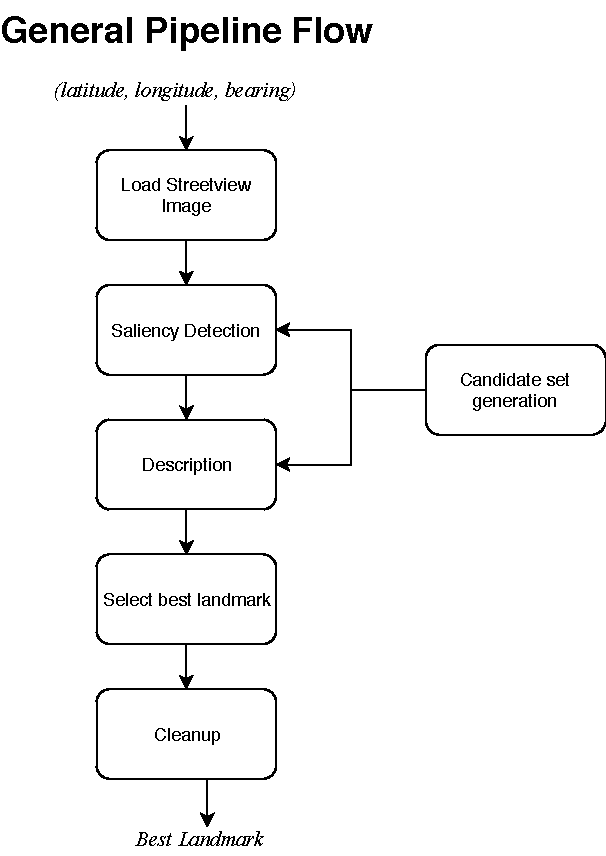
\includegraphics[width=0.6\textwidth]{pipeline_diagrams/general.pdf}
  \caption{The general structure of a Torchbearer pipeline.}
  \label{fig:pipeline:overview}
\end{figure}

While the exact manner in which a pipeline solves the landmark description problem varies from pipeline to pipeline, all pipelines share a general sequence of execution, and all take a tuple consisting of latitude, longitude and bearing as input and yield a tuple containing the best, most salient selected landmark as output.

The first step in any pipeline is to obtain a street-level image of the maneuver point at the given geographic coordinate and bearing (number 1 in Figure \ref{fig:pipeline:overview}). No matter the exact approach the pipeline takes to obtaining a landmark description, it will need this image to perform its determination. Next, the pipeline must generate a set of candidate landmarks, $C$. A candidate landmark is simply an object at the maneuver point that could be used as the basis for a landmark-based instruction; we know nothing about how salient the landmark is, however. 
	
Generation of the candidate landmark set is performed implicitly by either the saliency or description step, depending on the specific pipeline. Pipelines which leverage human-based description rely on the saliency step (whether human or machine-based) to generate a candidate set (step 2 in Figure \ref{fig:pipeline:overview}). Pipelines which use machine-based landmark description generate a candidate landmark set as part of the description step (step 3 in Figure \ref{fig:pipeline:overview}).

After the saliency of each candidate landmark has been determined (step 2 in Figure \ref{fig:pipeline:overview}), and each candidate has received a lexical description (step 3 in Figure \ref{fig:pipeline:overview}), the pipeline must decide which landmark is best, or most salient (step 4 in Figure \ref{fig:pipeline:overview}). The formula varies by pipeline, and depends on which components of saliency were measured.

\subsection{Saliency}
The saliency step of a pipeline is responsible for quantifying the saliency of candidate landmarks. While saliency consists of three components---visual, semantic and structural, not all three components are considered individually in each pipeline. Human-based saliency is based on only a single overall score, generated by human opinion, that represents humans' ability to distinguish good landmarks. Machine-based pipelines consider both semantic and visual saliency. In all pipelines, structural saliency is \textit{enforced} rather than \textit{evaluated}: in accordance with the literature, we consider only candidate landmarks that are located at or very near to the maneuver point.

\subsubsection{The Human Approach}
Humans are accustomed to picking out landmarks from their surroundings in day-to-day life, be it for giving a friend directions or for their own internalization of a route or location. We can take advantage of this innate ability by asking a human MTurk worker to select what they believe is the most salient, most standout landmark at a given maneuver point. Unlike algorithmic saliency detection, here we do not separate the concept of saliency into its visual and semantic subparts. Rather, we hypothesize that, because human workers have an elemental understanding of what makes a landmark salient, the decisions they make regarding the best landmark at a given point implicitly incorporate these saliency concepts.

We gather human saliency detection input via an MTurk HIT, denoted a ``Saliency HIT". The Saliency HIT must be completed by five workers, and consists of the following task: after the worker elects to work on the HIT, he is shown a high-resolution image of the maneuver point in question from three distances (at, just before, and before the point, corresponding to 10, 50, and 100 feet, respectively). Note that all three of these images are of equal dimensions. The HIT instructs the worker to use his mouse to draw a bounding box tightly around the object that he believes is the best landmark---the one he would use if he were telling a driver to perform the given maneuver right at that point. The worker can choose an object in any of the three images, but can only select one object.

We offer the worker three images from three distances so that landmarks of different scales can be captured: a stop sign, for example, is hard to detect in an image from far away, but is prevalent in an image from right near the maneuver point. Likewise, a large building may be an excellent landmark, but might only be visible from some distance away from the maneuver point. In essence, we are showing the worker the approach to, or the path leading up to, the landmark, and allowing them to see what the driver would see at three points along this path. In the final instruction spoken to the driver, we take into account the position of the best landmark---that is, if the best landmark is one which was selected from the “just before” image, the spoken instruction will tell the driver to turn “just after” the specified landmark.

After the worker makes his selection, the Torchbearer-hosted webpage submits the coordinates of the drawn bounding box, along with the position corresponding to the image the box was drawn in, to MTurk. After five workers complete the task, MTurk sends the set of five bounding boxes back to Turk Service, via a distributed queue. Torchbearer must now aggregate these answers: this particular human task leverages the “sampling and aggregation” approach to human input described in a previous section. That is, because bounding box coordinates are quantitative, we can combine them together in a manner which rewards the “agreement” among workers, if there is any, and culls answers which are in the severe minority and likely to be meaningless. 

Turk Service performs aggregation by creating a matrix called a \textit{saliency map} for each of three maneuver point images; this matrix represents the number of workers who included each pixel in the bounding box they drew. Algorithm \ref{alg:saliencyMap} creates this matrix. The result of this operation is a matrix of size equal to the maneuver point images shown to the worker, where an element corresponds to a pixel in the original maneuver point image and where the value of each element is an integer between 0 and $n$, where $n$ is equal to the number of workers. While the saliency map does not incorporate any decision about which regions are or are not salient landmarks, it encodes the relative saliency of each pixel in the image. To make this matrix easier to work with in subsequent pipeline steps, we normalize all values between 0 and 255, where a value of 255 indicates maximal saliency. A subsequent task in a pipeline can use this saliency map to either find the most salient regions or to query the total saliency of a target region.

\begin{algorithm}[htbp]
%\textbf{Algorithm} Compete
\textbf{Input}: $B$, a set of tuples $(x_1, y_1, x_2, y_2)$ representing bounding boxes;
$m$, the width of maneuver point image;
$n$, the height of maneuver point image; \\
\textbf{Output}: $S$, a matrix of dimension $m$ by $n$ 
\begin{algorithmic}[1]
\STATE $S\gets 0_{m,n}$
\FOR {$b \in B$}
    \STATE $S[b_{y1}:b_{y2}, b_{x1}:b_{x2}] \mathrel{+}= 1$
\ENDFOR
\RETURN{$B$}
\end{algorithmic}
\caption{Creating a saliency map from human input}\label{alg:saliencyMap}
\label{alg:saliencyMap}
\end{algorithm} 

\subsubsection{The Machine Approach}
The algorithmic approach to determining salient landmarks consists of separate components for visual and semantic saliency. However, the machine-based saliency step deals only with visual saliency; the machine-based description step provides semantic saliency scores.

Visual saliency refers to the perceptive quality of a region of the driver’s view which causes that region to stand out from its neighbors--that is, the degree to which a region grabs a driver’s visual attention. Street-level imagery of a maneuver point serves as input; the goal is to quantify each pixel of a maneuver point image in terms of its relative visual saliency. Specifically, given an $m$ x $n$ input image of a maneuver point, we output an $m$ x $n$ \textit{saliency map}, where each element in the matrix is an integer between 0 and 255 corresponding to how visually salient that pixel is. A value of 0 indicates no saliency, while a value of 255 indicates maximal saliency.

Torchbearer leverages a state-of-the art, deep-learning based algorithm called SalNet \cite{Pan_2016_CVPR} to estimate the pixel-level visual saliency across an image. Rather than seeking to identify specific neuroscience-inspired image features, which identify saliency, as many previous approaches do, SalNet takes a completely data-driven approach, using a deep convolutional neural network to “learn” where the human gaze tends to fixate in different images. Training data consists of a large dataset of ImageNet \cite{imagenet_cvpr09} images, each with a corresponding ground truth \textit{saliency map}. This dataset was created by tracking subjects' gaze as they were shown each image and recording the time gaze was focused on each pixel. These gaze times were then normalized to between 0 and 255, inclusive.

SalNet uses a deep neural network architecture to predict the saliency map for an input image. The first three layers of this network consist of pretrained layers from a Visual Geometry Group image classification network, VGG16 \cite{Simonyan14c}; the authors recognize that the low-level features learned by these layers offer valuable input to the saliency problem. VGG16 was trained on an extremely large dataset, and by using transfer learning, SalNet can benefit from this extensive training without needing to train on so many images itself. 

After the pretrained VGG network, SalNet incorporates a series of convolutional and pooling layers, and finally a deconvolutional layer, which will cast the output back into a matrix of the same size as the input. Training of the neural network consists of minimizing the Euclidean distance between the saliency map output by the network and the ground truth saliency map provided by the training dataset. During training, the weights of the first three layers are fixed at the pretrained weights from the VGG16 network; only the additional, saliency-specific layers unique to SalNet are actively trained.

It is important to note that SalNet is trained on a wide range of ImageNet images from across a broad range of topics; it does not incorporate any knowledge specific to the navigation domain. At the time of writing, no dataset containing ground truth saliency maps for street-level imagery of sufficient size for training a neural network was available. Training the SalNet architecture with domain-specific data would certainly be worthwhile future work. However, the general principles of visual saliency are not specific to any single domain, and the generalized training of SalNet allows it to perform well on an evaluation set of images from across the ImageNet corpora. We have hypothesized that it can adequately generalize to the navigation domain.

\begin{figure}[htbp]
  \centering
  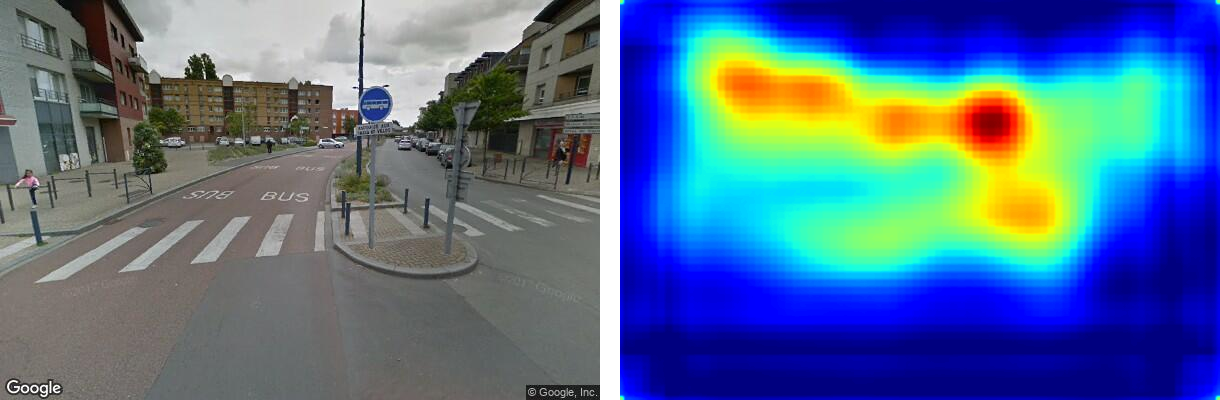
\includegraphics[width=0.6\textwidth]{images/saliencyMap.png}
  \caption{Left: a maneuver point image. Right: a corresponding saliency map generated by SalNet}
  \label{fig:saliencyMap}
\end{figure}

\subsection{Description}
The second half of the landmark selection problem consists of deriving a lexical description of a candidate landmark, although the machine approach to description is also responsible for generating candidate landmarks as well as providing semantic saliency scores. This description should be specific enough so as to allow a driver to easily distinguish that given landmark from its surroundings.

\subsubsection{The Human Approach}
To gather human descriptions for a given landmark, we again leverage Mechanical Turk. However, instead of using a sampling approach as we did with saliency crowdsourcing, we use a verification approach.
First, for a candidate landmark $c$, we annotate the street-level image of the maneuver point for which this landmark is a candidate to include a bounding box drawn around the landmark. We create an MTurk HIT is with only a single assignment; the worker is shown this image and asked to describe the object enclosed in the bounding box. The exact format of the question is: \texit{``Provide a specific description of the main object in the box. Describe PERMANENT, man-made things--NOT cars, people or things that could move. Pretend you were using that object as a landmark when giving someone directions."} The Torchbearer-hosted webpage presents the worker with a text box into which to type their answer.

After the worker has submitted the description, we create a verification HIT on MTurk, with three assignments. The annotated maneuver point image, along with the candidate description, is shown to each worker. The worker is asked to decide whether the description is accurate and meets the criteria of describing “permanent, man-made things--not cars, people or things that could move”. Three radio buttons are displayed—--``Description is accurate" and ``Description is inaccurate and the landmark is valid", and ``not a valid landmark".

If at least two of the three workers indicate that the description is accurate, the description is accepted, and pipeline execution can continue. If at least two of the three workers indicate the landmark is invalid, pipeline execution continues, with this landmark removed from the set of candidates. If the majority of workers indicate that the description is incorrect, or if there is no majority opinion, the description process repeats, with the creation of a new description HIT and subsequent verification HITs. Torchbearer will retry this process up to three times---if no description could be derived, the landmark is removed from the candidate set and pipeline execution continues.

\subsubsection{The Machine Approach}
Torchbearer leverages two approaches for finding semantically salient landmarks and quantifying their salience: a data driven approach, which uses a geosocial datasource to estimate the local significance of business and points of interest, and a deep learning-based object detection algorithm, which searches for known types of semantically salient features in maneuver point images.
	
\subsubsection{Data-driven Approach}
Torchbearer estimates the semantic saliency of a landmark via an estimate of the number of people, who have recently visited the landmark counted by the social networking application FourSquare. Previous work has shown the efficacy of using geosocial streams as a proxy for the local importance of a landmark; the intuition being that the more people who have “checked in” to a given location, the more well-known, or prominent, it is \cite{quesnot2014measure}. FourSquare incorporates businesses, points of interest and publicly accessible places into its ecosystem; these are referred to as venues. User location is recorded transparently, without the need for the user to explicitly tap a ``check in" button Torchbearer leverages FourSquare’s venue data both to find candidate landmarks and determine their semantic saliency. 

To find candidate landmarks for a given maneuver point, Torchbearer queries FourSquare for venues which are within a given radius of the maneuver point. By default, we use a small 100-foot radius, in the aim of ensuring any returned venue will be on or near the road upon which the maneuver point is located. FourSquare returns a list of tuples consisting of the venue name, the type of venue (such as restaurant, gas station, etc.) the geographic coordinates and the number of FourSquare users who have “checked in” to that venue. 

We compute the relative bearing between the venue and the approach bearing of the user, and discard venues which are not within 45-degrees of either side of the user, as the field-of-view of our street-level imagery is 90-degrees. We convert each of these venues to a Landmark: the landmark's description is the name of the FourSquare venue, concatenated with its category. For example, the description for a landmark corresponding to a venue with the name ``Starbucks" and category ``Coffee Shop" would be ``Starbucks Coffee Shop". The landmark’s semantic saliency score, $S_s$ is a function of the number of checkins in the last six months $c$ and the number of locations $l$, if the venue is a chain:
\begin{equation}
    S_s = c + l
\end{equation}

This measure captures both the local significance and wide-area ubiquity of the landmark. Note that all saliency scores are relative, and are meant to be compared against other candidate landmarks at a maneuver point.

\subsubsection{Object detection approach}
Some landmarks are ubiquitous and proven to be highly semantically salient, independent of the maneuver point's geographic location. Road infrastructure, such as stop signs and traffic lights, is a prime example: these landmarks are universally recognizable among drivers, and have been shown to serve as excellent landmarks for use in navigation instructions \cite{may_ross_bayer_2005}. Unfortunately, we found no dataset of street signage or traffic lights with coverage beyond a specific locality. Instead, we leverage a state-of-the-art object detection algorithm, Faster-RCNN \cite{ren2015faster}, to detect stop signs and traffic lights at maneuver points. Note that as a direction for future research, extending the object detection model to include other types of landmarks is both feasible and potentially beneficial.

Faster-RCNN (FRCNN) is a deep, region-based, convolutional neural network which takes an image as input and yields a set of bounding boxes, class labels (a string denoting which object the region was classified as) and confidence scores for objects of interest detected within the image\cite{ren2015faster}. It is currently one of the highest performing classifiers in terms of both speed and accuracy \cite{russakovsky2015imagenet}, \cite{ren2015faster}. 

FRCNN leverages an existing image classification network, ResNet, to compute feature maps for an image, and then uses the output of an intermediate convolutional layer in that base network as input to its own FRCNN-specific layers. This inclusion of a network trained for large-scale classification is known as transfer learning, and allows an FRCNN model to take advantage of the extensive training across millions of ImageNet images encoded within ResNet. The output of this intermediate convolutional layer, although trained on ImageNet data, outputs high-level image features as opposed to specific classes probabilities. Using these high-level feature maps as input, FRCNN trains its own final (fully-connected) layers to output class probabilities specific to our data.

FRCNN consists of two sub-networks: a Region Proposal Network (RPN), trained to output a set of possible bounding boxes, and the CNN network itself, which performs classification and final bounding box adjustment (based on the predicted class). To predict likely bounding boxes, the RPN considers a pre-generated set of \textit{anchor boxes}. Each anchor box is a fixed set of 9 candidate bounding boxes, of different sizes and aspect ratios, anchored at every point in the image. For example, if the input image is of dimensions $n$ x $n$, there are $9n^2$ anchor boxes for the RPN to consider. For each anchor box, the RPN learns to output (through the training of three convolutional layers) a probability corresponding to the likelihood of the box containing an object of interest, as well as a tuple of four doubles indicating the amount by which to adjust each coordinate of the predefined anchor box. Boxes with a probability of objectiveness below a certain threshold are discarded, the rest are passed on to the classification sub-network.

Given a set of possible bounding boxes generated by the RPN, the CNN first uses Region of Interest Pooling (ROI) to generate fixed-size convolutional feature maps corresponding to the region of the input feature map contained within each bounding box. ROI consists of splitting the box into $k$ evenly sized regions and selecting the maximal value from each region, yielding a feature map of size $k$, where $k$ is a small integer, often 7. This pooled feature map is then input to two successive 4096-neuron fully-connected layers--these two layers learn the actual classification function. 

The output of the second fully-connected layer is passed through a softmax layer of size equal to $c + 1$, where $c$ is the number of classes we are trying to predict. (The extra output is for the ``background" class--a bounding box that did not contain an object.)  The softmax layer gives a floating-point number for each output, subject to the following constraint: let $Y$ be the set of outputs, then 
\begin{equation}
    \sum\limits_{y \in Y} y = 1
\end{equation}

This gives a probability distribution over the set of possible classes for the likelihood of an object being a particular class (or background).

In addition to the softmax output corresponding to class predictions, the network outputs a tuple of bounding box adjustments corresponding to each class. (These are output via a single fully-connected layer of size $4c$.) These adjustments capture information about how to transform a pre-generated anchor box into the correct shape for a class; for example, it will learn that a stop sign is square.

Using images from Google Streetview, we constructed a dataset of 800 street-level images and ground-truth bounding boxes. Ground truth labels were created by hand using the Visual Object Tagging Tool \cite{vott}. Each image contained traffic lights, stopsigns or both. We generated an addition 75 negative examples---images containing neither a stoplight nor a stop sign. This dataset was divided into training and test sets, with a split of 85\% train and 15\% test. We trained an FRCNN network for 20 epochs--that is, 20 complete passes through our training set. At the completion of training, we achieved a mean average precision on our test dataset of 0.71 for stop lights and 0.75 for stop signs.

\subsection{Finding landmarks in saliency maps}
Given a saliency map, it is often important to locate candidate landmarks based on “hot spots”, or highly salient regions, in the map. The significance of this is different for human-based saliency detection than for machine-based saliency detection. As an example, consider the street-level image and corresponding saliency map shown in Figure \ref{fig:ws:ex}.

\begin{figure}[htbp]
  \centering
  \includegraphics[width=\textwidth]{ws_images/ws_ex.pdf}
  \caption{Left: a street-level image, with two stop signs and a building as potentially salient landmarks. Center: the corresponding saliency map, generated by SalNet. Right: the saliency map overlaid atop the street-level image.}
  \label{fig:ws:ex}
\end{figure}

With human-based saliency detection, the goal is to reduce the set of returned bounding boxes into a reduced set of distinct landmarks, by combining overlapping bounding boxes into a single area. For example, of the five answers it might be that three bounding boxes mostly overlap, indicating that that those workers intended to select the same landmark, while the other two answers overlap a separate landmark. Rather than treat all five bounding boxes as separate landmarks, it is beneficial to instead consider only the two distinct landmarks. First, this reduces the scale of future pipeline operations---those steps do not need to perform (redundant) calculations on as many candidate landmarks. This reduction saves time and compute cycles and, in the case of human-based tasks, fees paid to workers. Second, by reducing bounding boxes into aggregated areas, we can assign a saliency score to the candidate landmark based on how many answers included it in their bounding box. This can be used at the end of the pipeline as part of the decision process for choosing the best landmark. It is this score that acts as proxy for human intuition into what makes the best landmark: the more workers who select the pixels containing a landmark, the more salient the landmark.

In the case of machine-based candidate landmark generation, we need to correlate the set of candidate landmarks generated by the machine description (FourSquare-based) step with an area of the visual saliency map. Only the latitude, longitude and relative bearing between street-level image and landmark are known. We need to locate potential salient regions in the saliency map, so that we can determine if the candidate landmark aligns with one of those regions. 
Given a saliency map, a matrix of values ranging from 0 to 255, the goal is to label each pixel as belonging to a specific salient region or being non-salient. 

Non-maximal suppression (NMS) is a state-of-the-art method for reducing a set of bounding boxes to only the significant ones, discarding bounding boxes which enclose the same region using greedy clustering and a fixed distance threshold \cite{neubeck2006efficient}. If our saliency map were composed of entirely rectangular regions of different saliency values (as is actually the case with human-based saliency detection) this method would be sufficient. However, the saliency map returned by our computer-vision based saliency algorithm estimates saliency at the pixel level and, as a result, makes no guarantee about the shape of salient regions.

The Watershed Algorithm is an image segmentation approach, designed to single out distinct regions in the image by separating foreground elements from background elements \cite{barnes2014priority}. In classic image processing, these regions might be objects one wishes to separate from one another. In our case, we wish to separate regions of relatively high saliency (foreground) from their low-saliency surroundings (background). The algorithm works by considering our saliency map as a topological surface, where the value of a pixel denotes its height--pixels with a value of 0 (no saliency) are valleys and pixels with a value of 255 (highest saliency) are peaks. For each valley, or minima, in the map, the algorithm simulates filling the topology with different-colored water--that is, it labels pixels as belonging to a given segment. As simulated the water level rises, water from different valleys will begin to converge. To prevent this, the algorithm constructs infinitely tall barriers, or segmentation lines, between the two valleys. The algorithm continues this process until even the tallest peak is submerged, leaving only the barriers above water. These barriers now encapsulate different objects, or salient regions, within the map. 

To make this algorithm more impervious to over-segmentation and noise--small regions of high salience within a low-salience area or vise versa--we leverage the marker-controlled watershed algorithm \cite{roerdink2000watershed}. Here, we dictate to the algorithm which pixels we know to be independent, salient regions, which ones we know to be non-salient, background pixels and which ones we are unsure about (the border area between known salient regions and non-salient background). Now, rather than flooding starting at the minima, the algorithm begins flooding from each foreground region we specified and the background region; it is now simply finding where the segmentation line will be placed within the unknown border area.

In order to apply the watershed algorithm, several preprocessing morphological steps must be taken to “clean up” the saliency map, and each pixel must be labeled according to its status as known background, known foreground, or unknown. We adapt a procedure outlined in \cite{opencv_2017}. The following steps outline this process, given a saliency map $S$:

\begin{enumerate}
\item
Perform binary segmentation on $S$, rendering each pixel as salient (255) or non-salient (0). (This segmentation yields a ``black and white" image.) We first compute a threshold $t$, at or above which a pixel is considered salient and below which a pixel is considered non-salient. We select $t$ via Otsu Thresholding \cite{otsu1979threshold}, which works by iterating through all possible threshold values in $[0, 255]$ and selecting the one which minimizes the sum of the weighted variances within the salient and non-salient classes. That is,
\begin{equation}\label{eq:otsu}
    threshold=argmin_t(\frac{\mid n \mid}{\mid n \mid +\mid s \mid} \sigma_{n}^{t} + \frac{\mid s \mid}{\mid n \mid + \mid s \mid}\sigma_{n}^{t})
\end{equation}
where $t$ is the candidate threshold, $s$ is the set of salient pixels, $n$ is the set of non-salient pixels and $\sigma$ is the variance within the given set of pixels when a given $t$ is used as the threshold value. Figure \ref{fig:ws:thresh} shows the saliency map after Otsu Thresholding.

\begin{figure}[htbp]
  \centering
  
\includegraphics[width=0.5\textwidth]{ws_images/ws_thresh.png}
  \caption{The result of applying Otsu Thresholding to the saliency map. White areas (having a value of 255) represent areas of saliency.}
  \label{fig:ws:thresh}
\end{figure}

\item
Remove small, insignificant salient areas (white noise) by performing morphological opening on the binary segmentation. Figure \ref{fig:ws:open} shows the saliency map after applying morphological opening. While difficult to see at a small scale, several spots of white noise were removed.

\begin{figure}[htbp]
  \centering
  
\includegraphics[width=0.5\textwidth]{ws_images/ws_open.png}
  \caption{The saliency map after applying both Otsu Thresholding and morphological opening. While difficult to see at a small scale, several spots of white noise were removed.}
  \label{fig:ws:open}
\end{figure}

\item
Remove small, insignificant non-salient areas (holes) by performing morphological closing on the binary segmentation. Figure \ref{fig:ws:close} shows the results of this step; as this particular saliency map does not have any non-salient holes within a salient region the process had no visible effect.

\begin{figure}[htbp]
  \centering
  
\includegraphics[width=0.5\textwidth]{ws_images/ws_close.png}
  \caption{The results of the morphological closing step; as the particular saliency map does not have any non-salient holes within a salient region the process had no visible effect.}
  \label{fig:ws:close}
\end{figure}

\item
Determine which pixels are known to be non-salient by dilating the binary segmentation, falsely enlarging the salient regions. Dilation consists of scanning a square kernel $K$ over the binary segmentation and, at each point, replacing the binary segmentation pixel underneath the anchor point (center) of $K$ with the maximal value overlapped by $K$. Denote this dilation, shown in Figure \ref{fig:ws:bg}, as $M_n$.

\begin{figure}[htbp]
  \centering
  
\includegraphics[width=0.5\textwidth]{ws_images/ws_bg.png}
  \caption{Dilation $M_n$: the parts of the image known to be non-salient are in black (values of 0). Notice that the salient (white) regions are slightly enlarged compared to the results of the previous step.}
  \label{fig:ws:bg}
\end{figure}

\item
Apply a distance transformation to the binary segmentation, resulting in the value of each pixel being equal to the Euclidean distance between that pixel and a pixel with value 0 (non-salient background). This operation is essentially finding salient peaks, or the centers of salient regions, as the pixels which are farthest from a non-salient pixel are the ones in the center of a large salient region. Denote this distance transform as $D$ (shown in Figure \ref{fig:ws:dist}).

\begin{figure}[htbp]
  \centering
  
\includegraphics[width=0.5\textwidth]{ws_images/ws_dist.png}
  \caption{Distance transformation $D$: the center points of the salient regions are exactly white (255), as they are the farthest from a non-salient (black) pixel.}
  \label{fig:ws:dist}
\end{figure}

\item
Determine the set of pixels which are likely to be salient by applying a binary threshold to the distance transform, where $t$, the threshold, is set to $c * max(D)$, where $c$ is a constant factor which we set to 0.7. The goal is to isolate those pixels which are far from any non-salient pixels, as we can be confident that these are salient pixels. Denote this threshold $M_s$, shown in Figure \ref{fig:ws:fg}.

\begin{figure}[htbp]
  \centering
  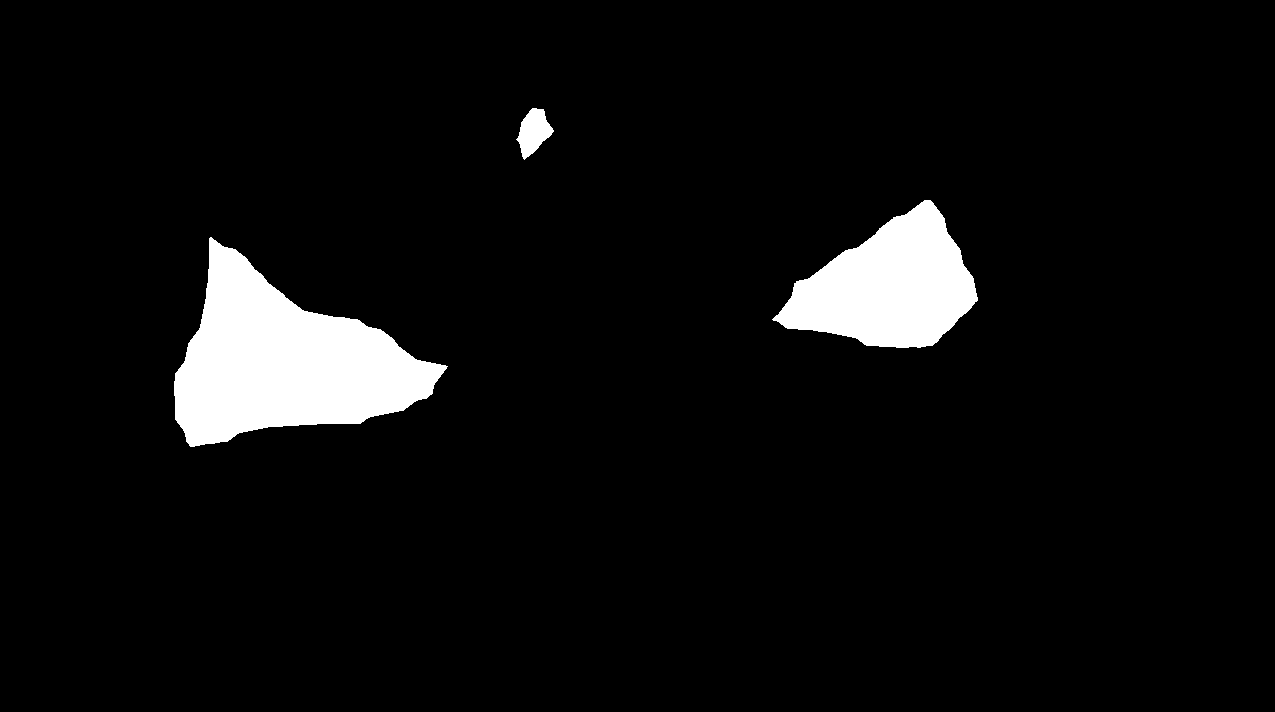
\includegraphics[width=0.5\textwidth]{ws_images/ws_fg.png}
  \caption{Threshold $M_s$, the white areas (values of 255) represent the areas of the saliency map we have high confidence are salient.}
  \label{fig:ws:fg}
\end{figure}

\item
Pixels which are not known to be either salient or non-salient can be found by $M_u = M_s - M_n$. This subtraction is shown in Figure \ref{fig:ws:unknown}.

\begin{figure}[htbp]
  \centering
  
\includegraphics[width=0.5\textwidth]{ws_images/ws_unknown.png}
  \caption{$M_u$, the result of subtracting the matrix of known background areas from the matrix of known foreground areas. the white areas (values of 255) represent the unknown areas between salient and non-salient (background) regions.}
  \label{fig:ws:unknown}
\end{figure}

\item
Each distinct (disconnected) region of salient pixels in $M_s$ needs to be labeled from $2...n+1$, where $n$ is the number of distinct regions. The background, or non-salient-pixels, must be labeled as 1. This is accomplished by performing a connected component analysis on $M_s$ with 8-connectivity, yielding $M_{labeled}$, a matrix with consecutively labeled connected components. (This matrix is shown in Figure \ref{fig:ws:unknown}.)
Label the unknown region with 0; this is the region in which watershed will draw a segmentation line to determine the final boundary around the salient regions. Specifically, $\forall p_{ij} \in M_u \mid p=0, M_l[i, j] = 0$.

\begin{figure}[htbp]
  \centering
  
\includegraphics[width=0.5\textwidth]{ws_images/ws_labeled.png}
  \caption{$M_{labeled}$, where dark blue is known non-salient background, purple is unknown, and yellow, green and turquoise are each a specific known salient region.}
  \label{fig:ws:labeled}
\end{figure}

\item
Run the watershed algorithm on $S$, using $M_{labeled}$ as markers. The returned matrix $M_w$ will have labeled all pixels as non-salient (1) or as belonging to a salient region (2...n+1). The result is shown in Figure \ref{fig:ws:ws}.

\begin{figure}[htbp]
  \centering
  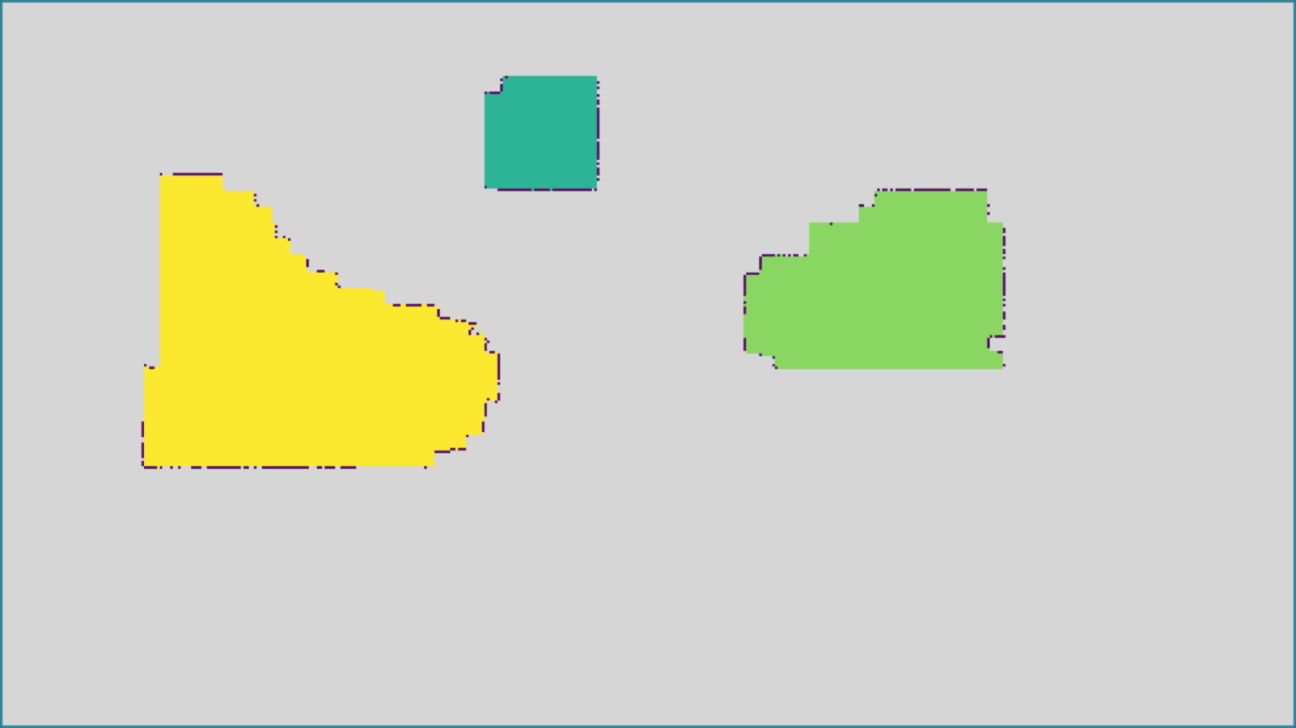
\includegraphics[width=0.5\textwidth]{ws_images/ws_ws.png}
  \caption{$M_{w}$, the result of the watershed algorithm. The grey region is non-salient background, and each of the colored regions is a distinct salient region.}
  \label{fig:ws:ws}
\end{figure}

\item
Calculate the bounding box around each salient region in $M_w$; these are the saliency map's salient regions. The final bounded salient regions are show in Figure \ref{fig:ws:bb}.

\begin{figure}[htbp]
  \centering
  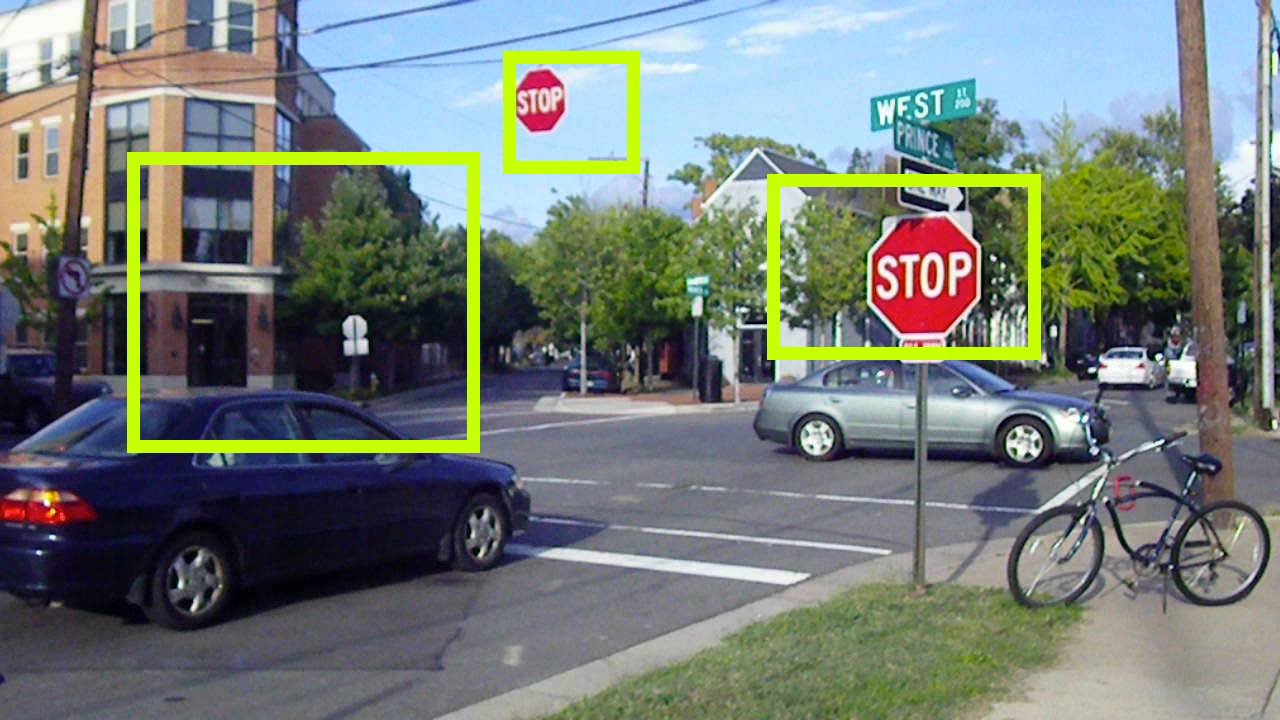
\includegraphics[width=0.5\textwidth]{ws_images/ws_bb.png}
  \caption{The final salient bounding boxes.}
  \label{fig:ws:bb}
\end{figure}

\end{enumerate}

\subsection{Quantifying Landmark Uniqueness}\label{sec:unique}

The semantic uniqueness of a landmark is an important factor in its saliency \cite{caduff2008assessment}. Even for pipelines that leverage human-based saliency detection, and therefore do not componentize the saliency score, uniqueness is still used for tie breaking purposes.

We use the lexical description of a landmark to derive its uniqueness as compared to the rest of the candidate landmark set. Our approach is based on word embeddings, where a word is represented as a high-dimensional vector in vector space \cite{goldberg2014word2vec}. The value in such a framework stems from the Distributional Hypothesis, which contends that words which are semantically similar will be distributionally similar as well, appearing together in the same written contexts \cite{harris1954distributional}. The goal in creating vectorizations of a set of words is to represent semantically similar words with similar, i.e. close, points in high-dimensional space. This approach allows us to determine the similarity of words by comparing the Euclidean distance between the points or cosine similarity between the corresponding (normalized) vectors.

\subsubsection{Word2Vec}
Predictive modeling is a common method for generating the vector representations of a set of words, wherein a machine learning algorithm learns to accurately predict a word's context, or words that are likely to appear around it, given only the word \cite{baroni2014don}. One such model, Word2Vec, is trained to predict a nearby word given another word, effectively internalizing a representation of which words appear in the same contexts \cite{mikolov2013efficient}. The algorithm uses a neural network with a single hidden layer of size equal to the desired dimensionality of the word embedding (often 300).  Using a large corpus of text, and a selected vocabulary of important words therein, the network is trained to accurately predict the probability of each word in the vocabulary occurring within a small window of other words in the vocabulary, within the text of the corpus. In doing so, the algorithm generates a $v$ x $d$ weight matrix (from the hidden layer to the output layer) which acts as a function from $word : P$, where $v$ is the size of the vocabulary, $d$ is the dimensionality of embeddings and $P$ is a vector of probabilities for each word in the vocabulary. After training, each row in this matrix represents the embedding for a word in the vocabulary. Intuitively, if two words are similar, they are likely to be surrounded by similar words, per the Distribution Hypothesis. Thus, they will have learned similar weights, so as to generate similar probability distributions over the vocabulary.

We use a pretrained word2vec model \cite{word2vec} with 300-dimensional word embeddings, trained on the Google News corpus and containing 300 million vocabulary words. We use cosine similarity as a measure of similarity between word embeddings, meaning that our similarity measure is bound between [-1, 1], with 1 indicating complete similarity and -1 indicting complete lack of similarity. 

To find the similarity between two landmark description phrases, we compute a description vector, which is a sum of the vectors of each word in a description. We then calculate the similarity between the two description vectors. Given two candidate landmarks $c_1$ and $c_2$, the similarity $s$ between these landmarks is defined as
\begin{equation}\label{eq:landmrkSimilarity}
    pairSimilarity = (c_1, c_2) \longrightarrow c(\sum\limits_{w \in c_1.description} embedding(w), \sum\limits_{w \in c_2.description} embedding(w))
\end{equation}
where $embedding$ is the word2vec vector for the given word and $c$ is the cosine similarity function of two vectors $v_1$ and $v_2$:
\begin{align}\label{eq:cosineSimilarity}
    c &= (v_1, v_2) \longrightarrow cos(\theta) \\
      &= (v_1, v_2) \longrightarrow \frac{A \cdot B}{\parallel A \parallel \parallel B \parallel}
\end{align}
where $\theta$ is the angle between the two vectors.

To find the similarity of a landmark $c$ as compared to all other landmarks in a set of candidate landmarks $C$:

\begin{equation}\label{eq:landmrkSimilarityOverall}
    totalSimilarity = \sum\limits_{k \in C} pairSimilarity(k, c)
\end{equation}

\section{Pipeline Specifics}
\subsection{Machine-Machine}

\noindent \textbf{Input}: $X_0 = (latitude, longitude, bearing)$\\
\textbf{Output}: The most salient landmark, including a description for use in navigation instructions\\
\textbf{Candidate selection}: Description

\begin{figure}[htbp]
  \centering
  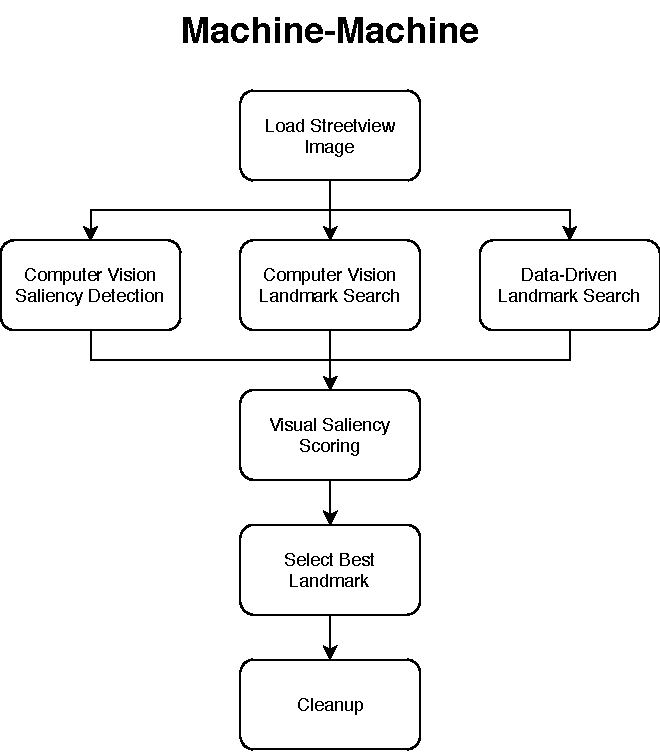
\includegraphics[width=0.6\textwidth]{pipeline_diagrams/machine-machine.pdf}
  \caption{The pipeline structure of the Machine-Machine pipeline.}
  \label{fig:pipeline:mm}
\end{figure}

\subsubsection*{Step 1: Load Streetview Image}~\\
\noindent \textbf{Input}: $X_0 = (latitude, longitude, bearing)$\\
\textbf{Output}: $Y_0 = (latitude, longitude, bearing, [image\_urls])$

This step consists of querying the Google Streetview API for street-level imagery at distances of 25, 50 and 100 feet from the given coordinate at an angle opposite of the bearing. (We refer to these distances relatively as “at”, “just before” and “before”.) Returned images are stored on Amazon Simple Storage Service (S3), and the S3 URL of each image is added to a tuple which is included in the output of this step. 

\subsubsection*{Step 2a: Computer Vision Saliency Detection}~\\
\noindent\textbf{Input}: $X_{2a} = Y_0 = (latitude, longitude, bearing, [image\_urls])$\\
\textbf{Output}: $Y_{2a} = (latitude, longitude, bearing, [image\_urls], [saliency\_matrices])$ 

Implementing the machine approach methodology outlined in the Saliency section, this step uses the SalNet deep learning architecture to compute a saliency map for each image in the tuple of images in $X_{2a}$. The processing of each image happens in parallel, and consists of feeding the the street-level image through SalNet and capturing the output.

For each image, this step yields a one-dimensional matrix of the same shape as the input image, with values ranging between 0 and 255, inclusive. Each matrix is included in the output tuple provided to subsequent pipeline steps.

\subsubsection*{Step 2b: Computer Vision Landmark Search}~\\
\noindent\textbf{Input}: $X_{2b} = Y_0 = (latitude, longitude, bearing, [image\_urls])$\\
\textbf{Output}: $Y_{2b} = (latitude, longitude, bearing,  [image\_urls], [candidate\_landmarks] )$ 

This step uses the Faster RCNN-based object recognition algorithm, described in the Saliency section, to detect candidate landmarks in each maneuver point image. The network has been trained to detect stop signs and stop lights; it returns, for each object it detects, a tuple consisting of the coordinates of the object’s bounding box within the image, a confidence score between 0 and 1 and a description (label) for the object. We discard any objects with a confidence score less than 0.8 based on the notion that it is better from a usability standpoint to not provide a landmark description in an instruction than it is to provide a description of a nonexistent landmark. The remaining objects are converted into candidate landmark tuples, with a semantic saliency score of 1.0. (We assume that all users are fully aware of what a stop sign or stoplight looks like, thus no other landmark can be more semantically salient than a landmark detected by this step.) These landmarks are included in the output of this step.

\subsubsection*{Step 2c: Data-driven Landmark Search}~\\
\textbf{Input}: $X_{2c} = Y_0 = (latitude, longitude, bearing, [image_urls])$\\
\noindent\textbf{Output}: $Y_{2c} = (latitude, longitude, bearing,$ \\ $[image\_urls], [candidate\_landmarks], [saliency\_matrices] )$

This step uses FourSquare to find candidate landmarks by searching for venues within a 100-foot radius of the maneuver point, as detailed in the Saliency section. Candidate landmarks are included in the output tuple.

\subsubsection*{Step 3: Visual Saliency Scoring}~\\
\textbf{Input}: $X_3 = Y_{2a} \cup Y_{2b} \cup Y_{2c} = (latitude, longitude, bearing,  [image\_urls],$\\ $[saliency\_maps], [candidate\_landmarks] )$\\
\noindent\textbf{Output}: $Y_3 = (latitude, longitude, bearing,  [image\_urls], [candidate\_landmarks] )$ 

This step assigns a quantitative score to each candidate landmark designating its visual saliency in the context of the maneuver point image. The computer-vision based saliency detection approach is not landmark-aware; that is, it determines relative saliency at the pixel-level. This step aggregates these pixel-level values into a score for the entire landmark. Given the bounding box coordinates $x_1, x_2, y_1,y_2$ of a candidate landmark and the saliency map $S$ of the maneuver point, the visual saliency score of that candidate is calculated as

\begin{equation}
    score= \frac{\sum\limits_{i=x_1}^{x_2} \sum\limits_{j=y_1}^{y_2} S_{ij}}{\sum S}
\end{equation}

That is, the visual saliency score is the sum of the submatrix contained within the bounding box divided by the sum of the entire saliency map. This gives two desirable properties: first, the larger a landmark is, the higher its score. Second, the more high-saliency pixels contained within a landmark bounding box, the higher its score.

While candidate landmarks detected by the object detection and human-based approaches include bounding boxes, and can therefore be correlated directly with a region in the saliency map, those returned by the data-driven approach do not. For these candidates, only the relative bearing between the maneuver point and landmark is known. In order to estimate which rectangular region of the saliency map corresponds to these landmarks we must first locate salient regions within the saliency map and then determine if one of those regions lies on the given bearing.

To locate salient regions, we use the watershed-based approach described previously. This lends us a set of bounding boxes, each containing a salient region within the saliency map. To determine if one of these salient regions represents our candidate landmark, we consider two points facts about the street-level image off of which the saliency map was created: first, the pitch of the image is zero degrees, meaning that the horizon line, where a venue would be, is roughly in the vertical middle of the image. Second, the field of view of the image is 90-degrees, and is not distorted or warped. Given the relative bearing between the maneuver point and the landmark, we check if there exists a salient region at this bearing in the vertical middle of the saliency map. (See Figure X.) If there is, we use this region as the bounding box for the candidate, and calculate the visual saliency score as above. If not, we assign a score of 0, as we have no evidence as to the visual saliency of this landmark.

\begin{figure}[htbp]
  \centering
  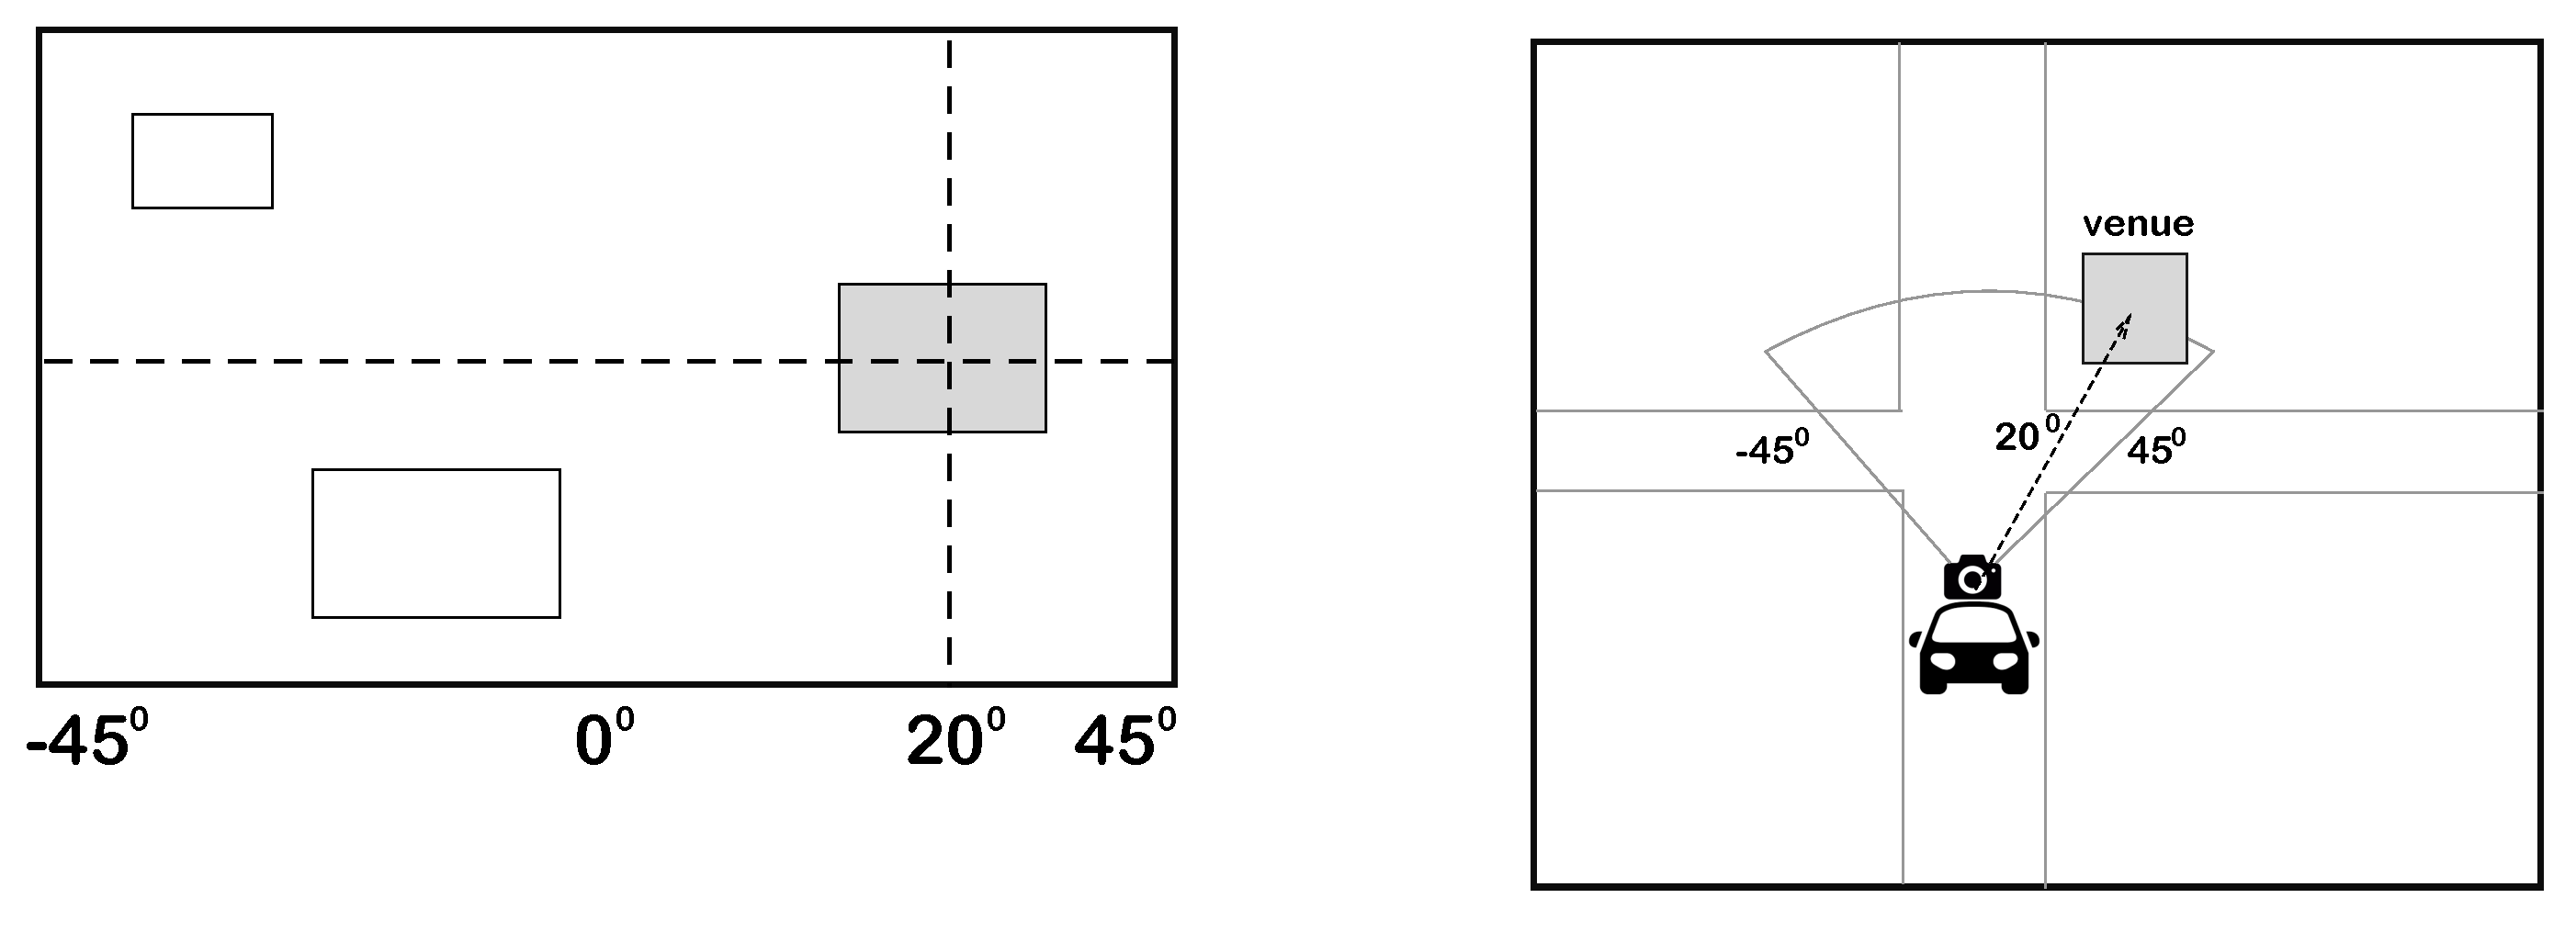
\includegraphics[width=0.6\textwidth]{images/landmark_search.pdf}
  \caption{Left: a landmark saliency map, with bounding boxes of salient regions. The intersection between the relative bearing parallel and vertical middle is within a salient region. Right: A bird's eye view of an intersection. Our street-level images are a rectilinear projection of a spherical image covering a 90 degree field of view.}
  \label{fig:pipeline:mm}
\end{figure}

\subsubsection*{Step 4: Select Most Salient Landmark}~\\
\noindent\textbf{Input}: $X_4 = Y_3 = (latitude, longitude, bearing,  [image\_urls],$\\ $[saliency\_maps], [candidate\_landmarks] )$\\
\textbf{Output}: $Y_4 = (latitude, longitude, bearing, best\_landmark)$ 

At this point in the pipeline, we have a set of candidate landmarks, each complete with both a visual and semantic saliency score. In order to determine the best, most salient landmark, we must first determine the uniqueness saliency score for each candidate, calculated via the method described in \ref{sec:unique}. Next, we normalize each of the three saliency scores to a value between 0 and 1. Given a set of candidate landmarks $C$, the normalized score for a given saliency component (visual, semantic or structural) for a given landmark $c$ can be found by

\begin{equation}
    score_{component} = \frac{c_{score}}{max_{i \in C}(i_{score})}
\end{equation}

The total saliency score for a candidate is then the sum of the three normalized scores. 

\begin{equation}\label{eq:saliency}
    S = S_v + S_s + S_u
\end{equation}

where $S_v$ is the visual saliency score, $S_s$ the semantic saliency score, and $S_u$ the uniqueness score, .

The candidate landmark with the highest summed scores is the best, most salient landmark, and is the output of this step. The description of this landmark will be included in navigation instructions spoken to the user.

\subsubsection*{Step 5: Cleanup}~\\
\noindent\textbf{Input}: $X_5 = Y_4 = (latitude, longitude, bearing, best\_landmark)$\\
\textbf{Output}: $Y_5 = (best\_landmark)$

This final step consists of system cleanup tasks. All intermediate images stored on S3 are removed--namely, street level imagery. The best landmark is stored in a database, associated with the maneuver point and pipeline identifier for future retrieval.

\subsection{Human-Machine}~\\
\noindent\textbf{Input}: $X_0 = (latitude, longitude, bearing)$\\
\noindent\textbf{Output}: The most salient landmark, including a description for use in navigation instructions\\
\textbf{Candidate selection}: Description

\begin{figure}[htbp]
  \centering
  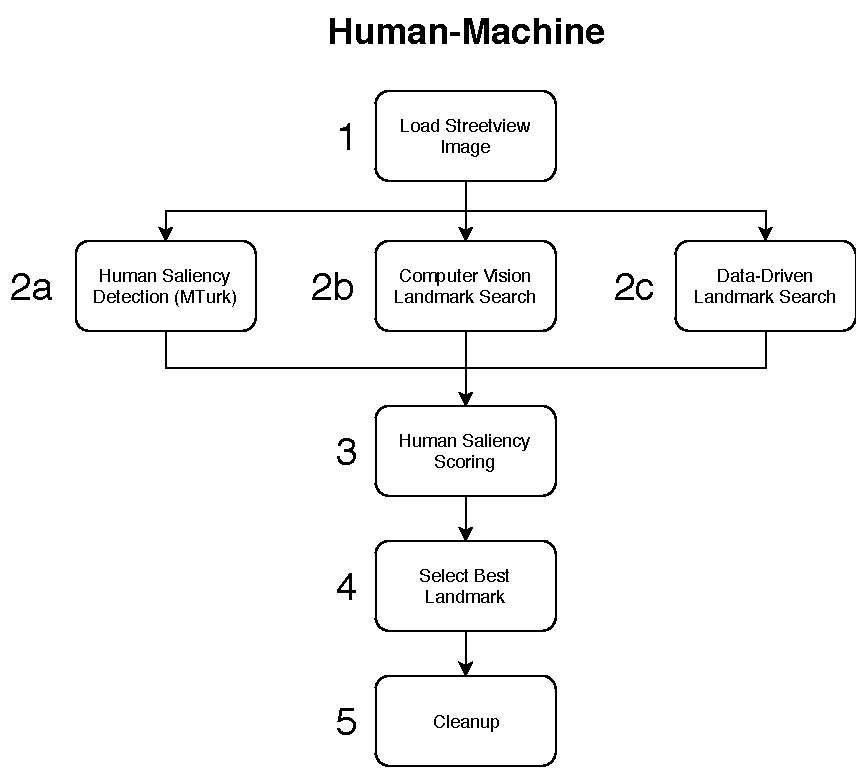
\includegraphics[width=0.6\textwidth]{pipeline_diagrams/human-machine.pdf}
  \caption{The pipeline structure of the Human-Machine pipeline.}
  \label{fig:pipeline:hm}
\end{figure}

\subsubsection*{Step 1: Load Streetview Image}~\\
\noindent\textbf{Input}: $X_1 = X_0 = (latitude, longitude, bearing)$\\
\textbf{Output}: $Y_1 = (latitude, longitude, bearing, [image\_urls])$

This step is implemented in the same manner as Step 1 of the Machine-Machine pipeline.

\subsubsection*{Step 2a: Human Saliency Detection}~\\ 
\noindent\textbf{Input}: $X_{2a} = Y_1 = (latitude, longitude, bearing, [image\_urls])$\\
\textbf{Output}: $Y_{2a} = (latitude, longitude, bearing, [image\_urls], [saliency\_matrices])$ 

This step generates a saliency matrix for the maneuver point, based off of the street-level image. This implementation uses the crowdsourcing approach described in the Saliency section, and leverages human intuition about what constitutes a good landmark. The saliency map generated is therefore not specific to a single component of landmark saliency (visual, semantic or structural) but comprises the entire saliency metric. 

The output of this step is a matrix of the same dimensions as the input maneuver point image; each element is a value between 0 and 255 indicating the relative saliency at that point in the image.

\subsubsection*{Step 2b: Computer Vision Landmark Search}~\\
\noindent\textbf{Input}: $X_{2b} = Y_1 = (latitude, longitude, bearing, [image\_urls])$\\
\textbf{Output}: $Y_{2b} = (latitude, longitude, bearing,  [image\_urls], [candidate\_landmarks] )$ 

This step is implemented in the same manner as Step 2b of the Machine-Machine pipeline.

\subsubsection*{Step 2c: Data-driven Landmark Search}~\\
\noindent\textbf{Input}: $X_{2c} = Y_1 = (latitude, longitude, bearing, [image\_urls])$\\
\textbf{Output}: $Y_{2c} = (latitude, longitude, bearing,  [image\_urls], $\\$[candidate\_landmarks], [saliency\_matrices] )$ 

This step is implemented in the same manner as Step 2c of the Machine-Machine pipeline.

\subsubsection*{Step 3: Visual Saliency Scoring}~\\
\noindent\textbf{Input}: $X_3 = Y_{2a} \cup Y_{2b} \cup Y_{2c} = (latitude, longitude, bearing,  [image\_urls],$\\$ [saliency\_maps], [candidate\_landmarks] )$\\
\textbf{Output}: $Y_3 = (latitude, longitude, bearing,  [image\_urls], [candidate\_landmarks] )$ 

This step is implemented in the same manner as Step 3 of the Machine-Machine pipeline.

\subsubsection*{Step 4: Select Most Salient Landmark}~\\
\noindent\textbf{Input}: $X_4 = Y_3 = (latitude, longitude, bearing,  [image\_urls], $\\$[saliency\_maps], [candidate\_landmarks] )$\\
\textbf{Output}: $Y_4 = (latitude, longitude, bearing, best\_landmark)$
 
The candidate landmark with the highest human saliency score is the best, most salient landmark, and is the output of this step. The description of this landmark will be included in navigation instructions spoken to the user.

\subsubsection*{Step 5: Cleanup}~\\
\noindent\textbf{Input}: $X_5 = Y_4 = (latitude, longitude, bearing, best_landmark)$\\
\textbf{Output}: $Y_5 = (best\_landmark)$

This step is implemented in the same manner as Step 5 of the Machine-Machine pipeline.

\subsection{Machine-Human}
\noindent\textbf{Input}: $X_0 = (latitude, longitude, bearing)$\\
\noindent\textbf{Output}: The most salient landmark, including a description for use in navigation instructions\\
\noindent\textbf{Candidate selection}: Saliency

\begin{figure}[htbp]
  \centering
  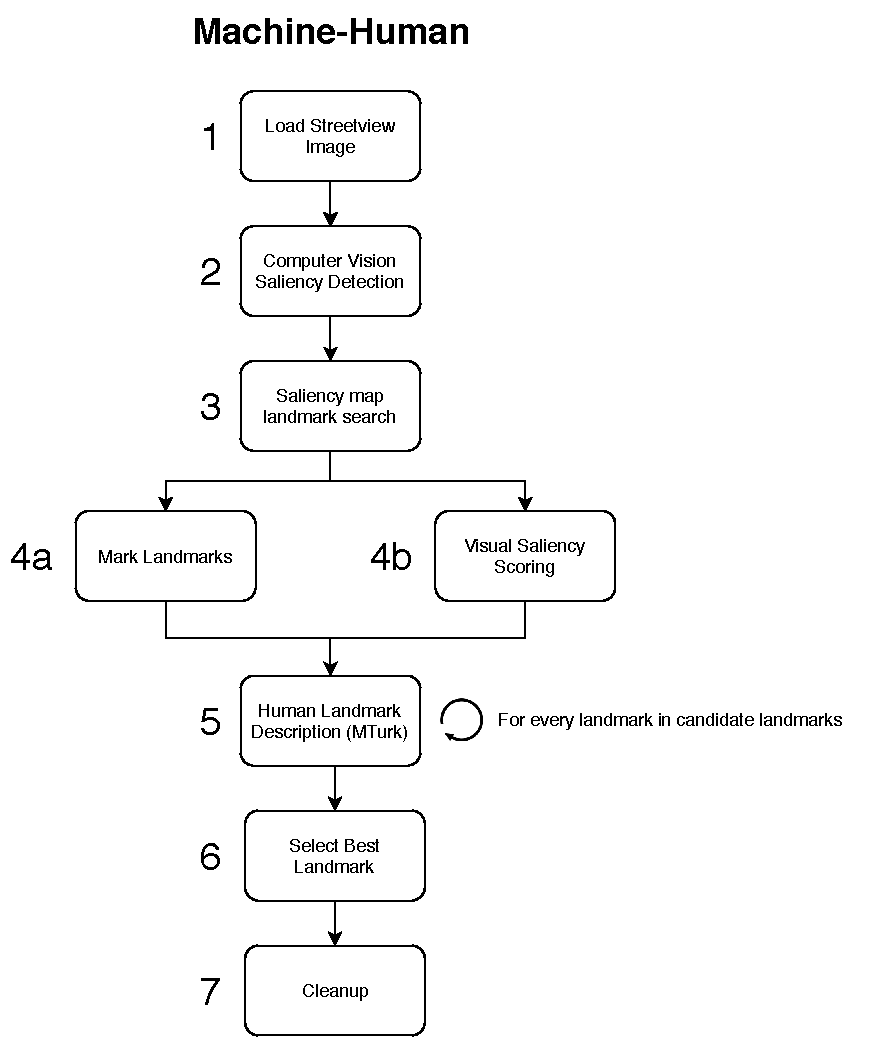
\includegraphics[width=0.6\textwidth]{pipeline_diagrams/machine-human.pdf}
  \caption{The pipeline structure of the Machine-Human pipeline.}
  \label{fig:pipeline:mh}
\end{figure}

\subsubsection*{Step 1: Load Streetview Image}~\\
\noindent\textbf{Input}: $X_1 = X_0 = (latitude, longitude, bearing)$\\
\textbf{Output}: $Y_1 = (latitude, longitude, bearing, [image\_urls])$

This step is implemented in the same manner as Step 1 of the Machine-Machine pipeline.

\subsubsection*{Step 2: Computer Vision Saliency Detection}~\\
\noindent\textbf{Input}: $X_2 = Y_0 = (latitude, longitude, bearing, [image\_urls])$\\
\textbf{Output}: $Y_2 = (latitude, longitude, bearing, [image\_urls], [saliency\_matrices])$ 

This step is implemented in the same manner as Step 2a of the Machine-Machine pipeline.

\subsubsection*{Step 3a: Create annotated maneuver point images}~\\
\noindent\textbf{Input}: $X_{3a} = Y_2 = (latitude, longitude, bearing, [image\_urls], [saliency\_matrices])$ \\
\textbf{Output}: $Y_{3a} = (latitude, longitude, bearing, [image\_urls],$\\$ [saliency\_matrices], [annotated\_image\_urls])$ 

In order for human workers to provide written descriptions for candidate landmarks, they need to see an image of the maneuver point with the candidate landmark outlined. We choose to show workers an annotated image of the entire maneuver point, as opposed to a cropped image containing only the candidate landmark, so that workers can incorporate context into their descriptions. For example, we have observed descriptions such as “one story blue house next to the oak tree” and “stop sign near the crosswalk”.

For each candidate $c$ in the set of candidate landmarks $C$, we generate an image which contains a 3-pixel thick red border drawn around the bounding box of $c$. These images are stored on S3, and the URLs are included in the output of this step.

\subsubsection*{Step 3b: Visual Saliency Scoring}~\\
\noindent\textbf{Input}: $X_{3b} = Y_2 = (latitude, longitude, bearing,  [image\_urls], $\\$[saliency\_maps], [candidat\_landmarks] )$\\
\textbf{Output}: $Y_{3b} = (latitude, longitude, bearing,  [image\_urls], [candidate\_landmarks] )$ 

This step is implemented in the same manner as Step 3 of the Machine-Machine pipeline, except that the landmark search (watershed) component is not needed as all candidate landmarks include bounding boxes.

\subsubsection*{Step 4: Human-based Landmark Description}~\\
\noindent\textbf{Input}: $X_4 = Y_{3a} \cup Y_{3b} = (latitude, longitude, bearing, $\\$[image\_urls], [saliency\_matrices], [annotated\_image\_urls])$ \\
\textbf{Output}: $Y_4 = (latitude, longitude, bearing, [image\_urls],$\\$ [saliency\_matrices], [annotated\_image\_urls])$ 

For each landmark $c$ in the set of candidate landmarks $C$, we utilize the human-based description method described in the Saliency section to obtain a lexical description of $c$. These descriptions are included in the given candidate landmark tuple in the output of this step. This step does not complete until all candidate landmarks have been processed through MTurk.

\subsubsection*{Step 5: Select Most Salient Landmark}~\\
\noindent\textbf{Input}: $X_5 = Y_4 = (latitude, longitude, bearing,  [image\_urls], $\\$[saliency\_maps], [candidate\_landmarks] )$\\
\textbf{Output}: $Y_5 = (latitude, longitude, bearing, best\_landmark)$
 
This step is implemented in the same manner as Step 4 of the Machine-Machine pipeline.

\subsubsection*{Step 6: Cleanup}~\\
\noindent\textbf{Input}: $X_6 = Y_5 = (latitude, longitude, bearing, best\_landmark)$\\
\textbf{Output}: $Y_6 = (best\_landmark)$

This step is implemented in the same manner as Step 5 of the Machine-Machine pipeline.

\subsection{Human-Human}
\noindent\textbf{Input}: $X_0 = (latitude, longitude, bearing)$\\
\textbf{Output}: The most salient landmark, including a description for use in navigation instructions\\
\textbf{Candidate selection}: Description

\begin{figure}[htbp]
  \centering
  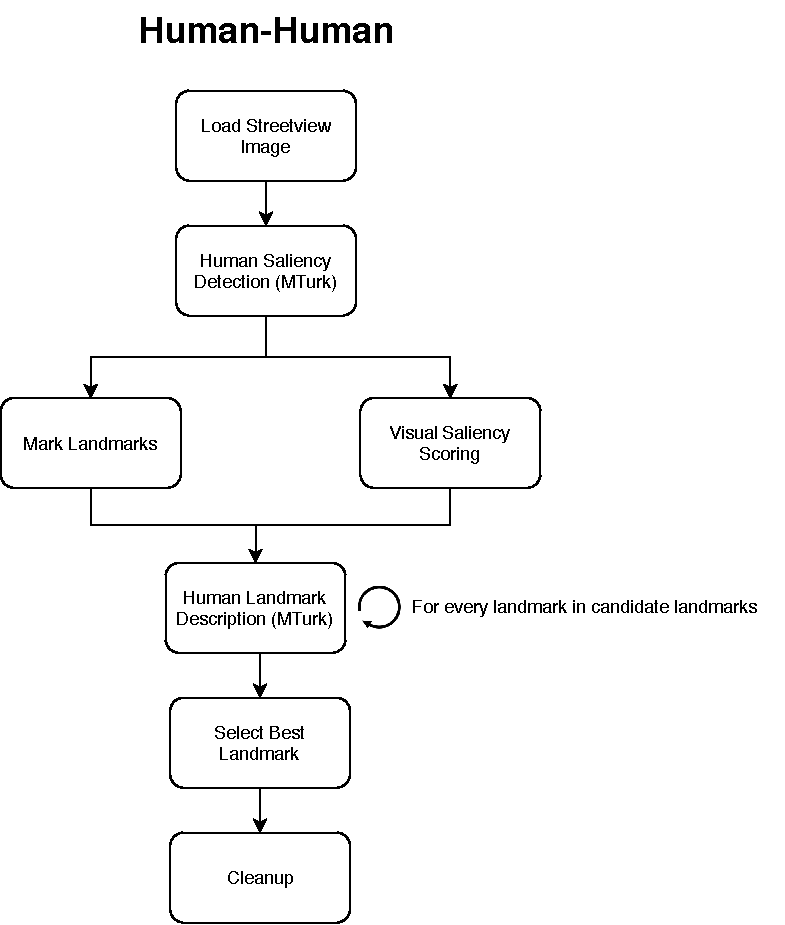
\includegraphics[width=0.6\textwidth]{pipeline_diagrams/human-human.pdf}
  \caption{The pipeline structure of the Human-Human pipeline.}
  \label{fig:pipeline:hh}
\end{figure}

\subsubsection*{Step 1: Load Streetview Image}~\\
\noindent\textbf{Input}: $X_1 = X_0 = (latitude, longitude, bearing)$\\
\textbf{Output}: $Y_1 = (latitude, longitude, bearing, [image\_urls])$

This step is implemented in the same manner as Step 1 of the Machine-Machine pipeline.

\subsubsection*{Step 2: Human Saliency Detection}~\\
\noindent\textbf{Input}: $X_{2} = Y_1 = (latitude, longitude, bearing, [image\_urls])$\\
\textbf{Output}: $Y_{2} = (latitude, longitude, bearing, [image\_urls], [saliency\_matrices])$ 

This step is implemented in the same manner as Step 2a of the Human-Machine pipeline.

\subsubsection*{Step 3a: Create annotated maneuver point images}~\\
\noindent\textbf{Input}: $X_{3a} = Y_2 = (latitude, longitude, bearing, [image\_urls], [saliency\_matrices])$ \\
\textbf{Output}: $Y_{3a} = (latitude, longitude, bearing, [image\_urls], $\\$[saliency\_matrices], [annotated\_image\_urls])$ 

This step is implemented in the same manner as Step 3a of the Machine-Human pipeline.

\subsubsection*{Step 3b: Visual Saliency Scoring}~\\
\noindent\textbf{Input}: $X_{3b} = Y_2 = (latitude, longitude, bearing, $\\$ [image\_urls], [saliency\_maps], [candidate\_landmarks] )$\\
\textbf{Output}: $Y_{3b} = (latitude, longitude, bearing,  [image\_urls], [candidate\_landmarks] )$ 

This step is implemented in the same manner as Step 3 of the Machine-Machine pipeline, except that the landmark search (watershed) component is not needed as all candidate landmarks include bounding boxes.

\subsubsection*{Step 4: Human-based Landmark Description}~\\
\noindent\textbf{Input}: $X_4 = Y_{3a} \cup Y_{3b} = (latitude, longitude, bearing, [image\_urls],$\\$ [saliency\_matrices], [annotated\_image\_urls])$ \\
\textbf{Output}: $Y_4 = (latitude, longitude, bearing, [image\_urls], $\\$[saliency\_matrices], [annotated\_image\_urls])$ 

This step is implemented in the same manner as Step 4 of the Machine-Human pipeline.

\subsubsection*{Step 5: Select Most Salient Landmark}~\\
\noindent\textbf{Input}: $X_5 = Y_4 = (latitude, longitude, bearing,  [image\_urls],$\\$ [salienc\y_maps], [candidate\_landmarks] )$\\
\textbf{Output}: $Y_5 = (latitude, longitude, bearing, best\_landmark)$
 
This step is implemented in the same manner as Step 4 of the Human-Machine pipeline.

\subsubsection*{Step 6: Cleanup}~\\
\noindent\textbf{Input}: $X_6 = Y_5 = (latitude, longitude, bearing, best\_landmark)$\\
\textbf{Output}: $Y_6 = (best\_landmark)$

This step is implemented in the same manner as Step 5 of the Machine-Machine pipeline.



